% Week 9: Decoding Strategies (Template Beamer Final Styling)
% BSc Discovery Two-Tier: 25 main + 19 appendix = 44 slides
% Professional lavender color scheme with 18pt+ fonts
% November 9, 2025

\documentclass[8pt,aspectratio=169]{beamer}
\usetheme{Madrid}
\usepackage{graphicx}
\usepackage{booktabs}
\usepackage{amsmath}
\usepackage{amssymb}

% Template Beamer Final Color Scheme
\definecolor{mlblue}{RGB}{0,102,204}
\definecolor{mlpurple}{RGB}{51,51,178}
\definecolor{mllavender}{RGB}{173,173,224}
\definecolor{mllavender2}{RGB}{193,193,232}
\definecolor{mllavender3}{RGB}{204,204,235}
\definecolor{mllavender4}{RGB}{214,214,239}
\definecolor{mlorange}{RGB}{255, 127, 14}
\definecolor{mlgreen}{RGB}{44, 160, 44}
\definecolor{mlred}{RGB}{214, 39, 40}
\definecolor{mlgray}{RGB}{127, 127, 127}

% Apply custom colors to Madrid theme
\setbeamercolor{palette primary}{bg=mllavender3,fg=mlpurple}
\setbeamercolor{palette secondary}{bg=mllavender2,fg=mlpurple}
\setbeamercolor{palette tertiary}{bg=mllavender,fg=white}
\setbeamercolor{palette quaternary}{bg=mlpurple,fg=white}

\setbeamercolor{structure}{fg=mlpurple}
\setbeamercolor{section in toc}{fg=mlpurple}
\setbeamercolor{title}{fg=mlpurple}
\setbeamercolor{frametitle}{fg=mlpurple,bg=mllavender3}
\setbeamercolor{block title}{bg=mllavender2,fg=mlpurple}
\setbeamercolor{block body}{bg=mllavender4,fg=black}

% Remove navigation symbols
\setbeamertemplate{navigation symbols}{}

% Clean itemize/enumerate
\setbeamertemplate{itemize items}[circle]
\setbeamertemplate{enumerate items}[default]

% Reduce margins
\setbeamersize{text margin left=5mm,text margin right=5mm}

% Bottom note with lavender separator
\newcommand{\bottomnote}[1]{%
\vfill
\vspace{-2mm}
\textcolor{mllavender2}{\rule{\textwidth}{0.4pt}}
\vspace{1mm}
\footnotesize
\textbf{#1}
}

% Math commands
\newcommand{\given}{\mid}
\newcommand{\argmax}{\operatorname{argmax}}
\newcommand{\softmax}{\operatorname{softmax}}

\title{Decoding Strategies}
\subtitle{Week 9: From Prediction to Generation}
\author{NLP Course 2025}
\institute{Enhanced with Contrastive Search (2025)}
\date{November 9, 2025}

\begin{document}

% ============================================
% MAIN PRESENTATION (25 SLIDES)
% ============================================

\begin{frame}[plain]
\titlepage
\vfill
\begin{center}
\small
\textcolor{mlpurple}{\textbf{Two-Tier BSc Discovery}}\\
\textcolor{mlgray}{Main: 25 slides | Appendix: 19 slides}
\end{center}
\end{frame}

% === CONTEXT: HOW WE GOT HERE (2 SLIDES) ===

\begin{frame}[t]{How We Got Here: The Prediction Story}
\vspace{-0.3cm}
\begin{center}
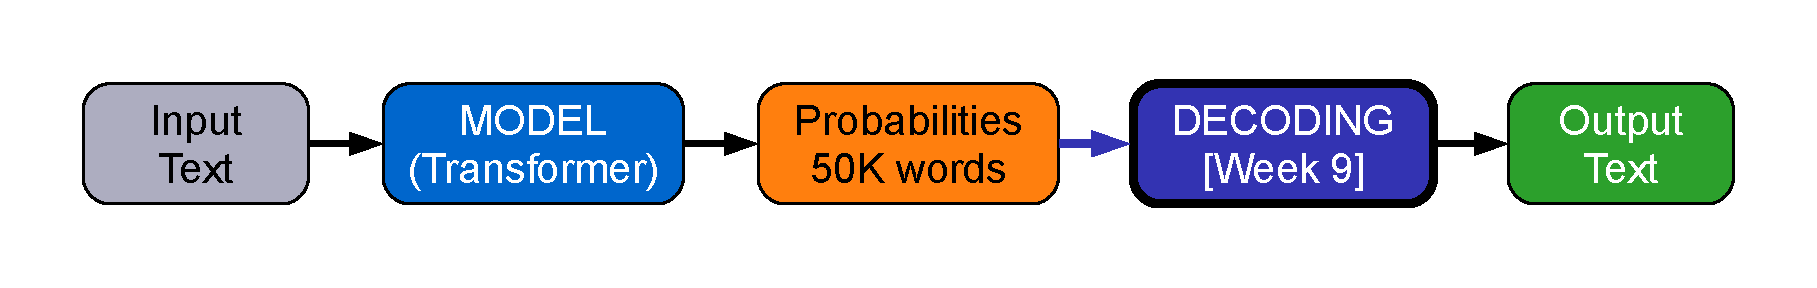
\includegraphics[width=0.75\textwidth]{../figures/prediction_to_text_pipeline_bsc.pdf}
\end{center}

\vspace{2mm}
\small
\textbf{Our Journey}:
\begin{enumerate}
\item We trained models (Weeks 3-7: RNN → Transformers → BERT/GPT)
\item They learned to predict: $P(\text{word} | \text{context})$
\item They output probability distributions over 50,000+ words
\item \textbf{Today}: How do we convert these probabilities into actual text?
\end{enumerate}

\bottomnote{Models predict probabilities. Decoding converts probabilities to text.}
\end{frame}

\begin{frame}[t]{Today's Challenge: From Probabilities to Text}
\small
\textbf{The Setup}: Model gives us probabilities for next word

\vspace{2mm}
Example: ``The cat \_\_''

$$P(\text{sat}) = 0.45, \quad P(\text{is}) = 0.30, \quad P(\text{jumped}) = 0.25, \quad ... \quad \text{(50,000 words)}$$

\vspace{3mm}
\begin{columns}[T]
\column{0.48\textwidth}
\textbf{Naive Approach 1}: Pick highest

$\rightarrow$ \textbf{Greedy Decoding}

\vspace{2mm}
\textbf{Result}:

\colorbox{mllavender4}{\parbox{0.90\textwidth}{
``The city is a major city in the city...''
}}

\vspace{2mm}
{\color{mlred}\textbf{Problem}}: Repetitive, boring

\column{0.48\textwidth}
\textbf{Naive Approach 2}: Pick random

$\rightarrow$ \textbf{Pure Sampling}

\vspace{2mm}
\textbf{Result}:

\colorbox{mllavender4}{\parbox{0.90\textwidth}{
``The purple flying mathematics...''
}}

\vspace{2mm}
{\color{mlred}\textbf{Problem}}: Nonsense, incoherent
\end{columns}

\vspace{3mm}
\begin{center}
\colorbox{mllavender2}{\parbox{0.85\textwidth}{
\centering
\textcolor{mlpurple}{\textbf{Core Challenge}}: Need text that is \textit{coherent} AND \textit{creative}
}}
\end{center}

\bottomnote{Today: 6 strategies to solve this - from simple to sophisticated}
\end{frame}

% === QUALITY-DIVERSITY HOOK (2 SLIDES) ===

\begin{frame}[t]{The Quality-Diversity Tradeoff}
\vspace{-0.3cm}
\begin{center}
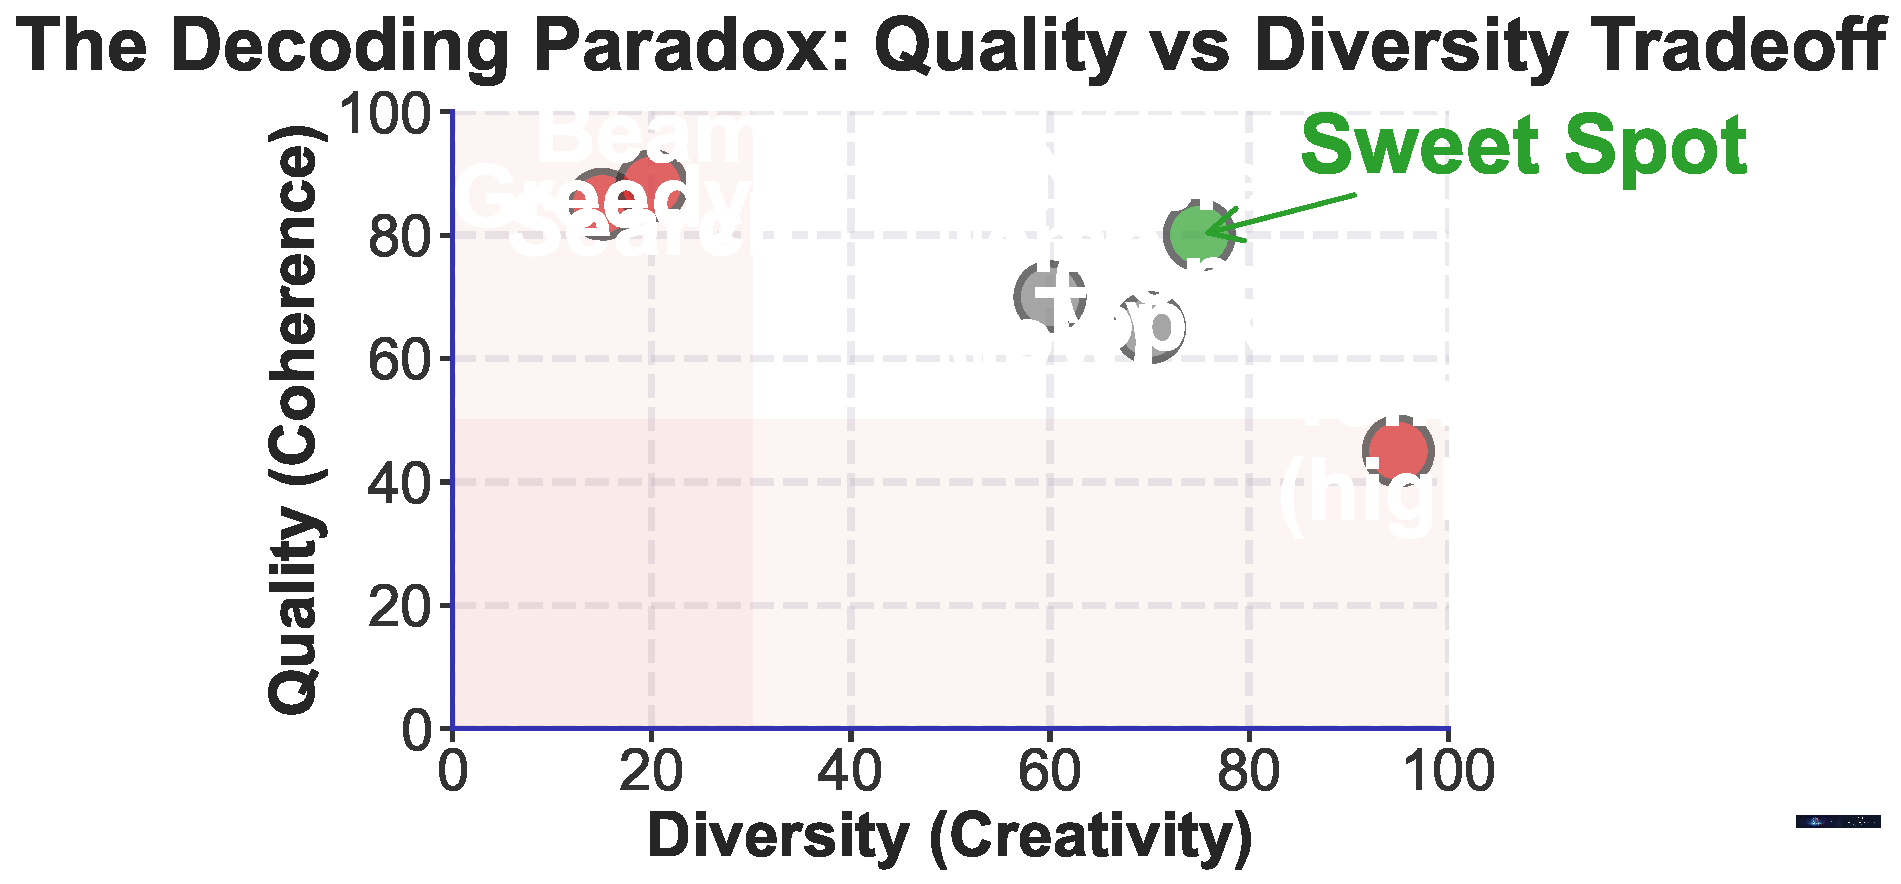
\includegraphics[width=0.70\textwidth]{../figures/quality_diversity_tradeoff_bsc.pdf}
\end{center}
\begin{center}
\colorbox{mllavender3}{\parbox{0.75\textwidth}{
\centering
\textcolor{mlpurple}{\textbf{Discovery Question}}: Why is best text boring and creative text nonsense?
}}
\end{center}
\bottomnote{The central challenge: How to balance coherence with creativity}
\end{frame}

\begin{frame}[t]{Three Decoding Families}
\small
\begin{columns}[T]
\column{0.32\textwidth}
\begin{block}{Deterministic}
\textbf{Methods}:
\begin{itemize}
\item Greedy
\item Beam search
\end{itemize}

\vspace{2mm}
\textbf{Traits}:
\begin{itemize}
\item Same output
\item High quality
\item No creativity
\end{itemize}
\end{block}

\column{0.32\textwidth}
\begin{block}{Stochastic}
\textbf{Methods}:
\begin{itemize}
\item Temperature
\item Top-k
\item Nucleus
\end{itemize}

\vspace{2mm}
\textbf{Traits}:
\begin{itemize}
\item Random
\item Creative
\item Variable quality
\end{itemize}
\end{block}

\column{0.32\textwidth}
\begin{block}{Balanced}
\textbf{Methods}:
\begin{itemize}
\item Contrastive
\item Hybrid
\end{itemize}

\vspace{2mm}
\textbf{Traits}:
\begin{itemize}
\item Best of both
\item No repetition
\item Modern std
\end{itemize}
\end{block}
\end{columns}

\vspace{3mm}
\begin{center}
\colorbox{mllavender3}{\parbox{0.85\textwidth}{
\centering
Different tasks need different strategies - no single best method
}}
\end{center}

\bottomnote{6 methods total: Each optimizes different quality-diversity tradeoff}
\end{frame}

% === DETERMINISTIC METHODS (4 SLIDES) ===

\begin{frame}[t]{Greedy Decoding: The Baseline}
\small
\begin{columns}[T]
\column{0.49\textwidth}
\textbf{How It Works}:

\begin{enumerate}
\item Compute probabilities
\item Pick highest probability
\item Add to sequence
\item Repeat until done
\end{enumerate}

\vspace{2mm}
\textbf{Example}:

\colorbox{mllavender4}{\parbox{0.85\textwidth}{
$P(\text{cat}) = 0.45$ ← Pick!

$P(\text{dog}) = 0.30$

$P(\text{bird}) = 0.25$
}}

\column{0.49\textwidth}
\textbf{When to Use}:
\begin{itemize}
\item Code generation
\item Short responses
\item Speed critical
\item Reproducibility
\end{itemize}

\vspace{2mm}
\colorbox{mlred!20}{\parbox{0.85\textwidth}{
\textbf{Problem: Degeneration}

``The city is a city in a city...''

Model gets stuck in loops
}}

\end{columns}
\bottomnote{Simplest but prone to repetition}
\end{frame}

\begin{frame}[t]{Beam Search: Explore Multiple Paths}
\vspace{-0.3cm}
\begin{center}
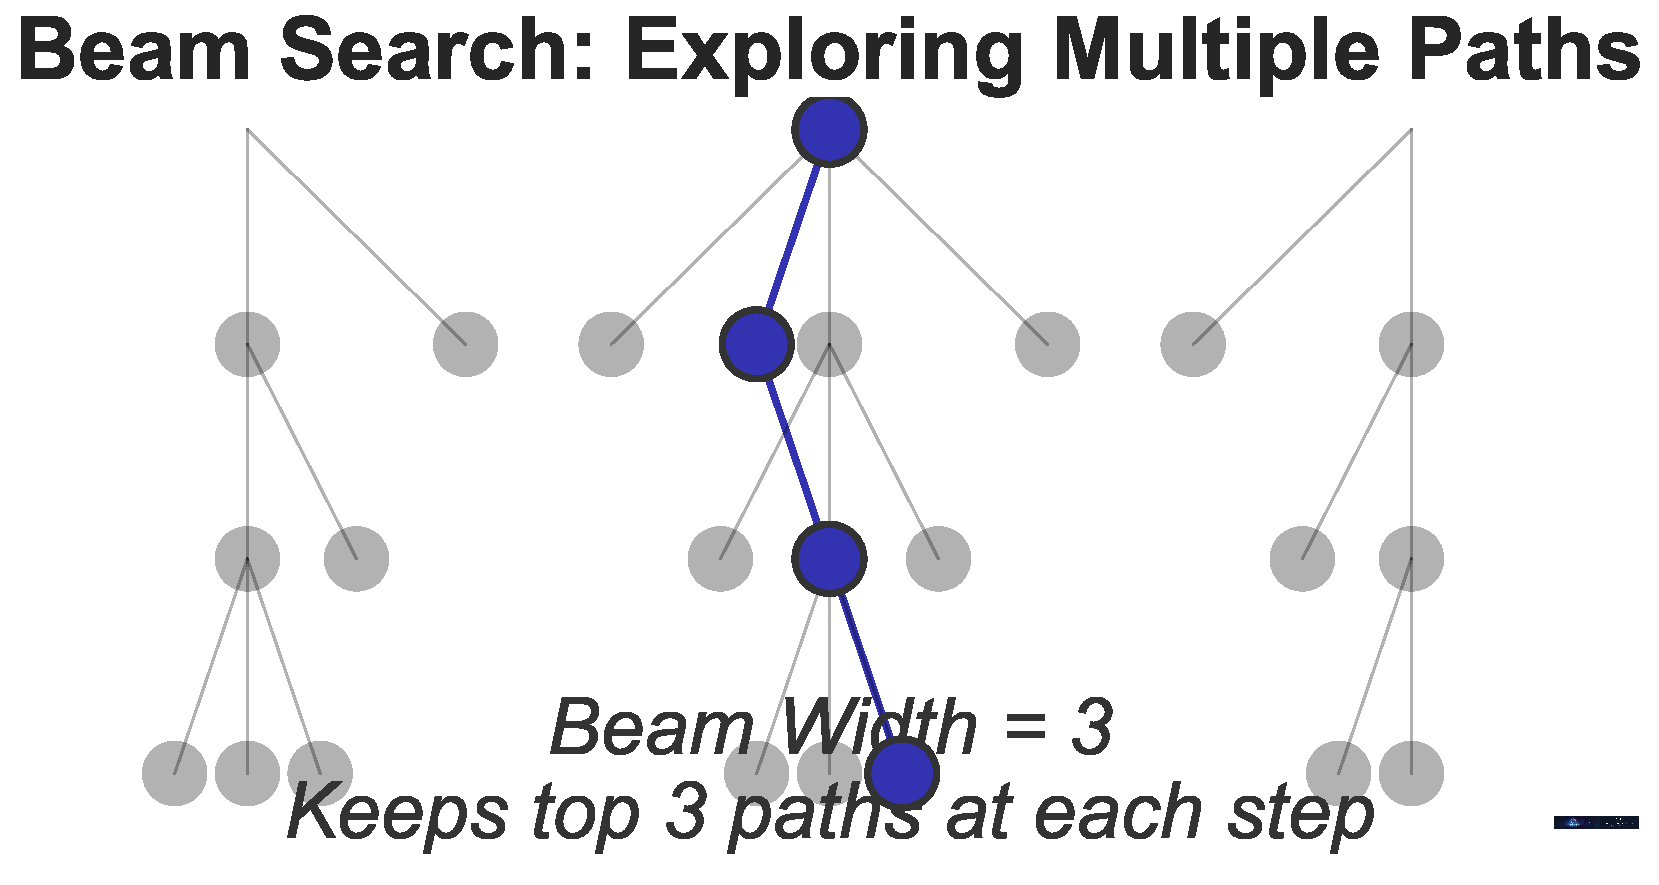
\includegraphics[width=0.70\textwidth]{../figures/beam_search_visual_bsc.pdf}
\end{center}
\begin{center}
\colorbox{mllavender3}{\parbox{0.80\textwidth}{
\centering
\textcolor{mlpurple}{\textbf{Key Insight}}: Keep top-k hypotheses at each step to find better sequences
}}
\end{center}
\bottomnote{Beam width = 3-5 typical. Balance greedy (1) vs exhaustive ($\infty$)}
\end{frame}

\begin{frame}[t]{Beam Search: Step-by-Step Example}
\vspace{-0.3cm}
\begin{center}
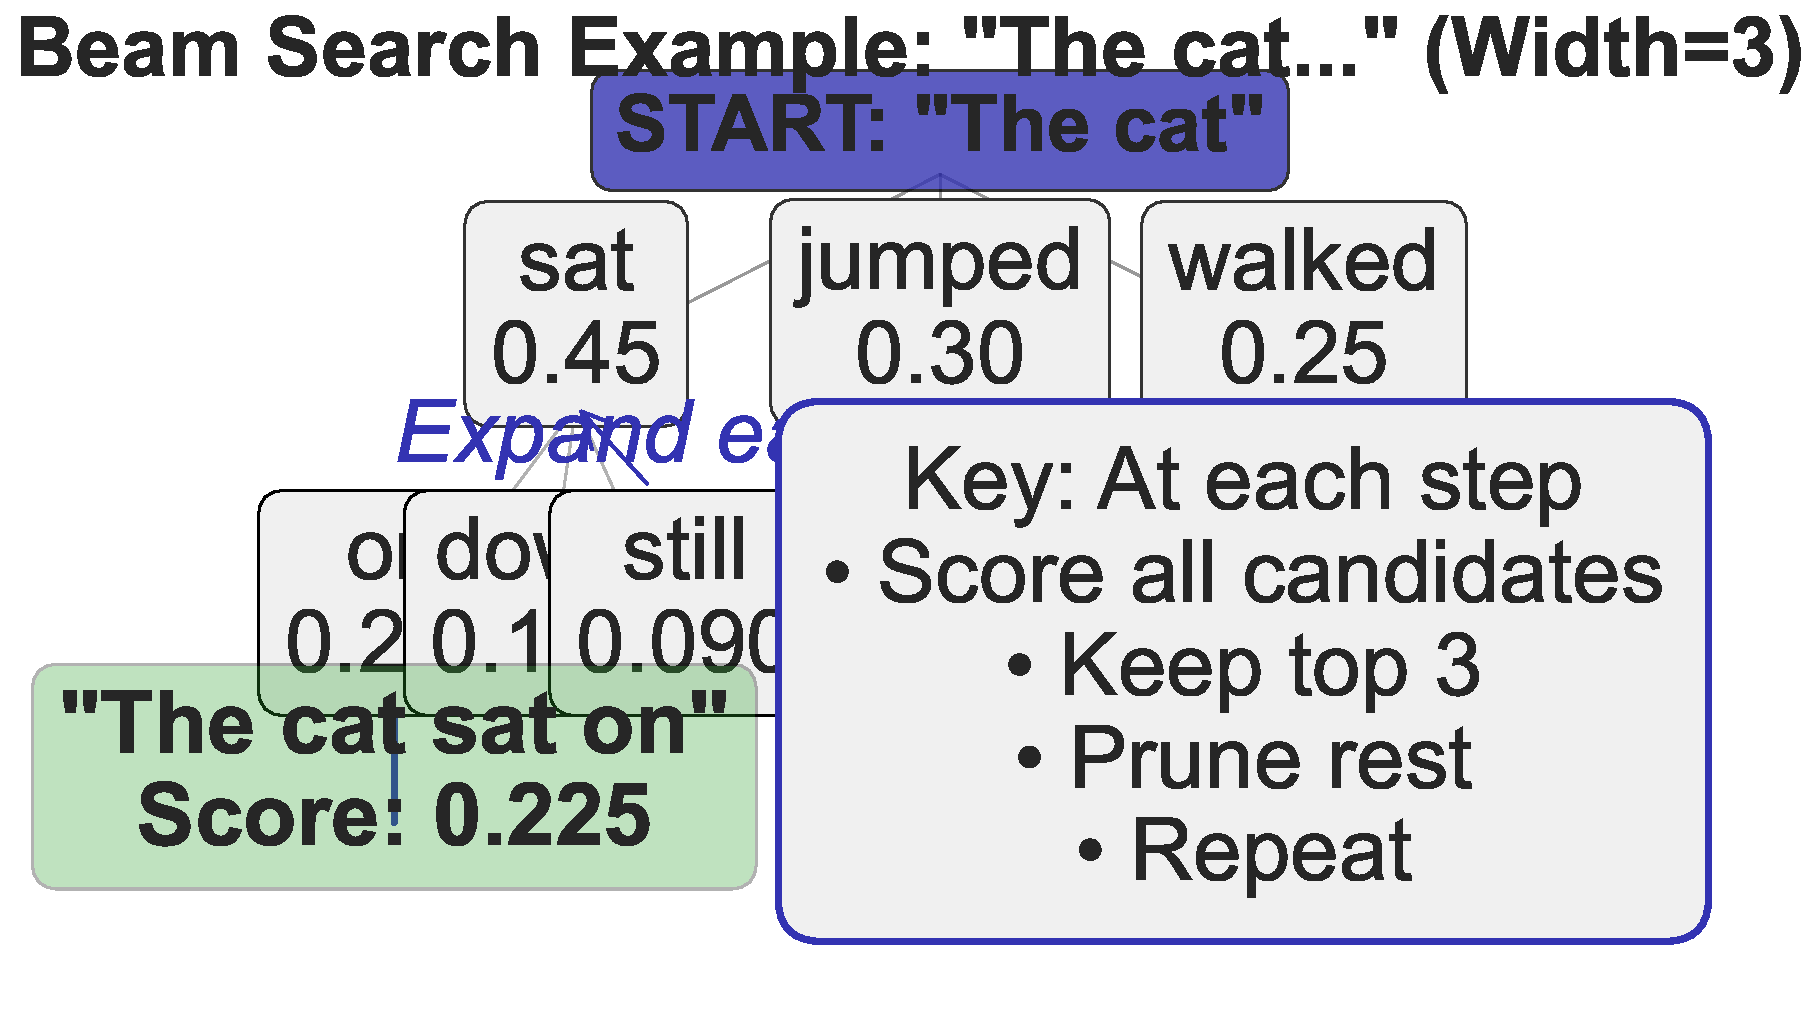
\includegraphics[width=0.75\textwidth]{../figures/beam_example_tree_bsc.pdf}
\end{center}
\bottomnote{Worked example: ``The cat...'' with width=3 shows pruning in action}
\end{frame}

\begin{frame}[t]{Beam Search: Detail}
\small
\begin{columns}[T]
\column{0.49\textwidth}
\textbf{Algorithm}:

\begin{enumerate}
\item Start: Keep top-k tokens
\item Expand: All continuations
\item Score: Multiply probs
\item Prune: Keep top-k sequences
\item Repeat until END
\end{enumerate}

\vspace{2mm}
\textbf{Scoring}:

$$\text{score} = \prod_{i=1}^t P(y_i | y_{<i})$$

With length normalization:

$$\text{score} = \frac{1}{t} \sum_{i=1}^t \log P(y_i | y_{<i})$$

\column{0.49\textwidth}
\textbf{Best For}:
\begin{itemize}
\item Machine translation
\item Summarization
\item Question answering
\item ``Correct'' answer tasks
\end{itemize}

\vspace{2mm}
\textbf{Parameters}:

Width = 3-5 (translation)

Width = 10 (more diverse)

\vspace{2mm}
\colorbox{mlgreen!20}{\parbox{0.90\textwidth}{
+ Better than greedy

+ Diverse hypotheses

- Still deterministic

- 4-5× slower
}}

\end{columns}
\bottomnote{Beam search: workhorse for deterministic tasks}
\end{frame}

% === STOCHASTIC METHODS (8 SLIDES) ===

\begin{frame}[t]{Temperature Sampling: Control Randomness}
\vspace{-0.3cm}
\begin{center}
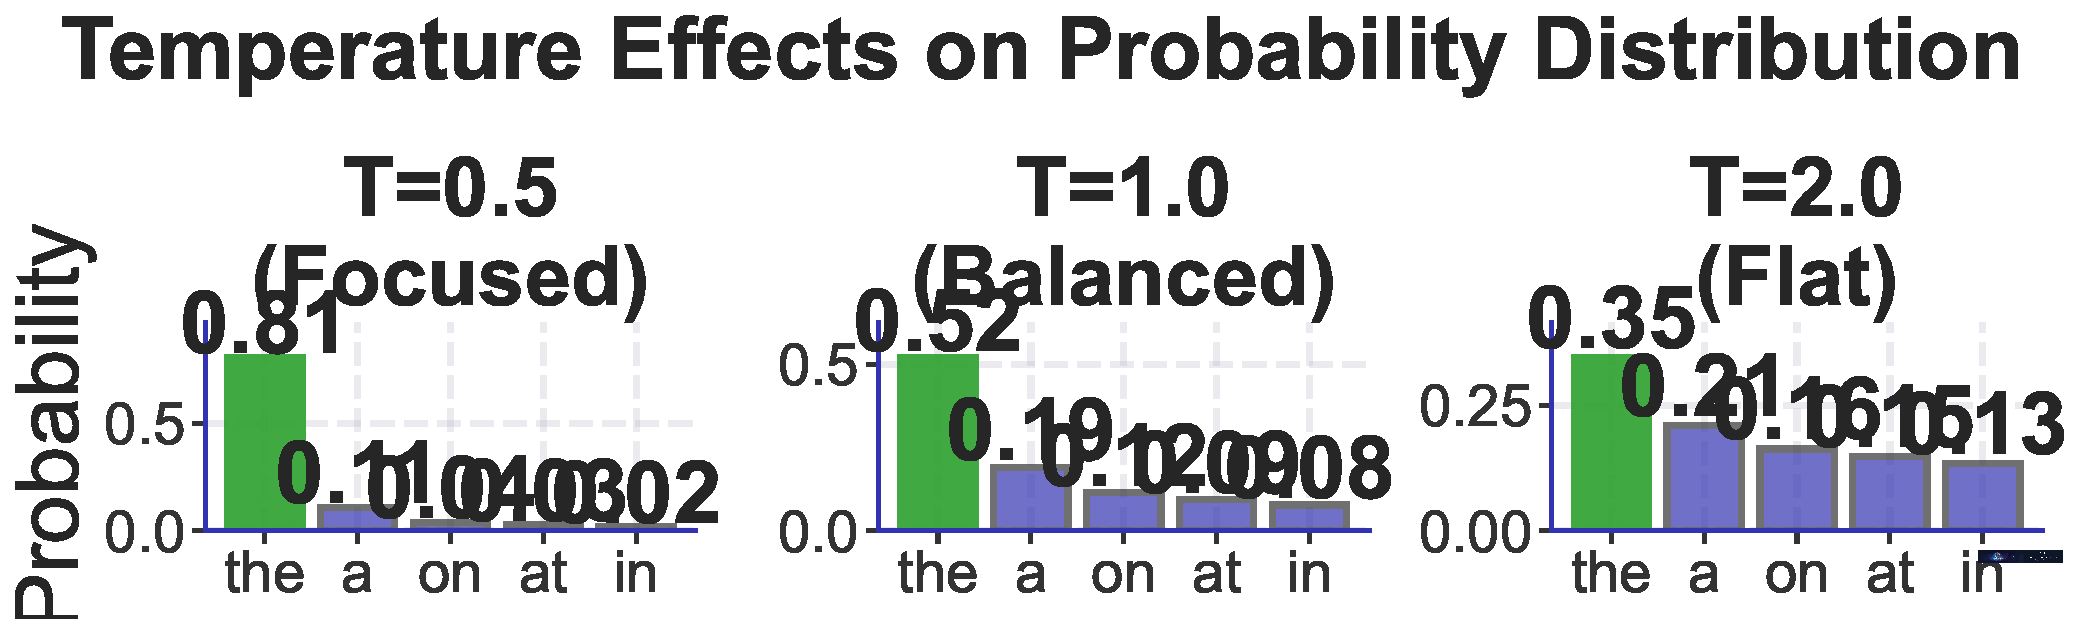
\includegraphics[width=0.65\textwidth]{../figures/temperature_effects_bsc.pdf}
\end{center}
\begin{center}
\colorbox{mllavender3}{\parbox{0.75\textwidth}{
\centering
\textcolor{mlpurple}{\textbf{Key Insight}}: Temperature reshapes probability distribution
}}
\end{center}
\bottomnote{T $<$ 1: focused. T = 1: unchanged. T $>$ 1: random}
\end{frame}

\begin{frame}[t]{Temperature: Worked Example}
\vspace{-0.3cm}
\begin{center}
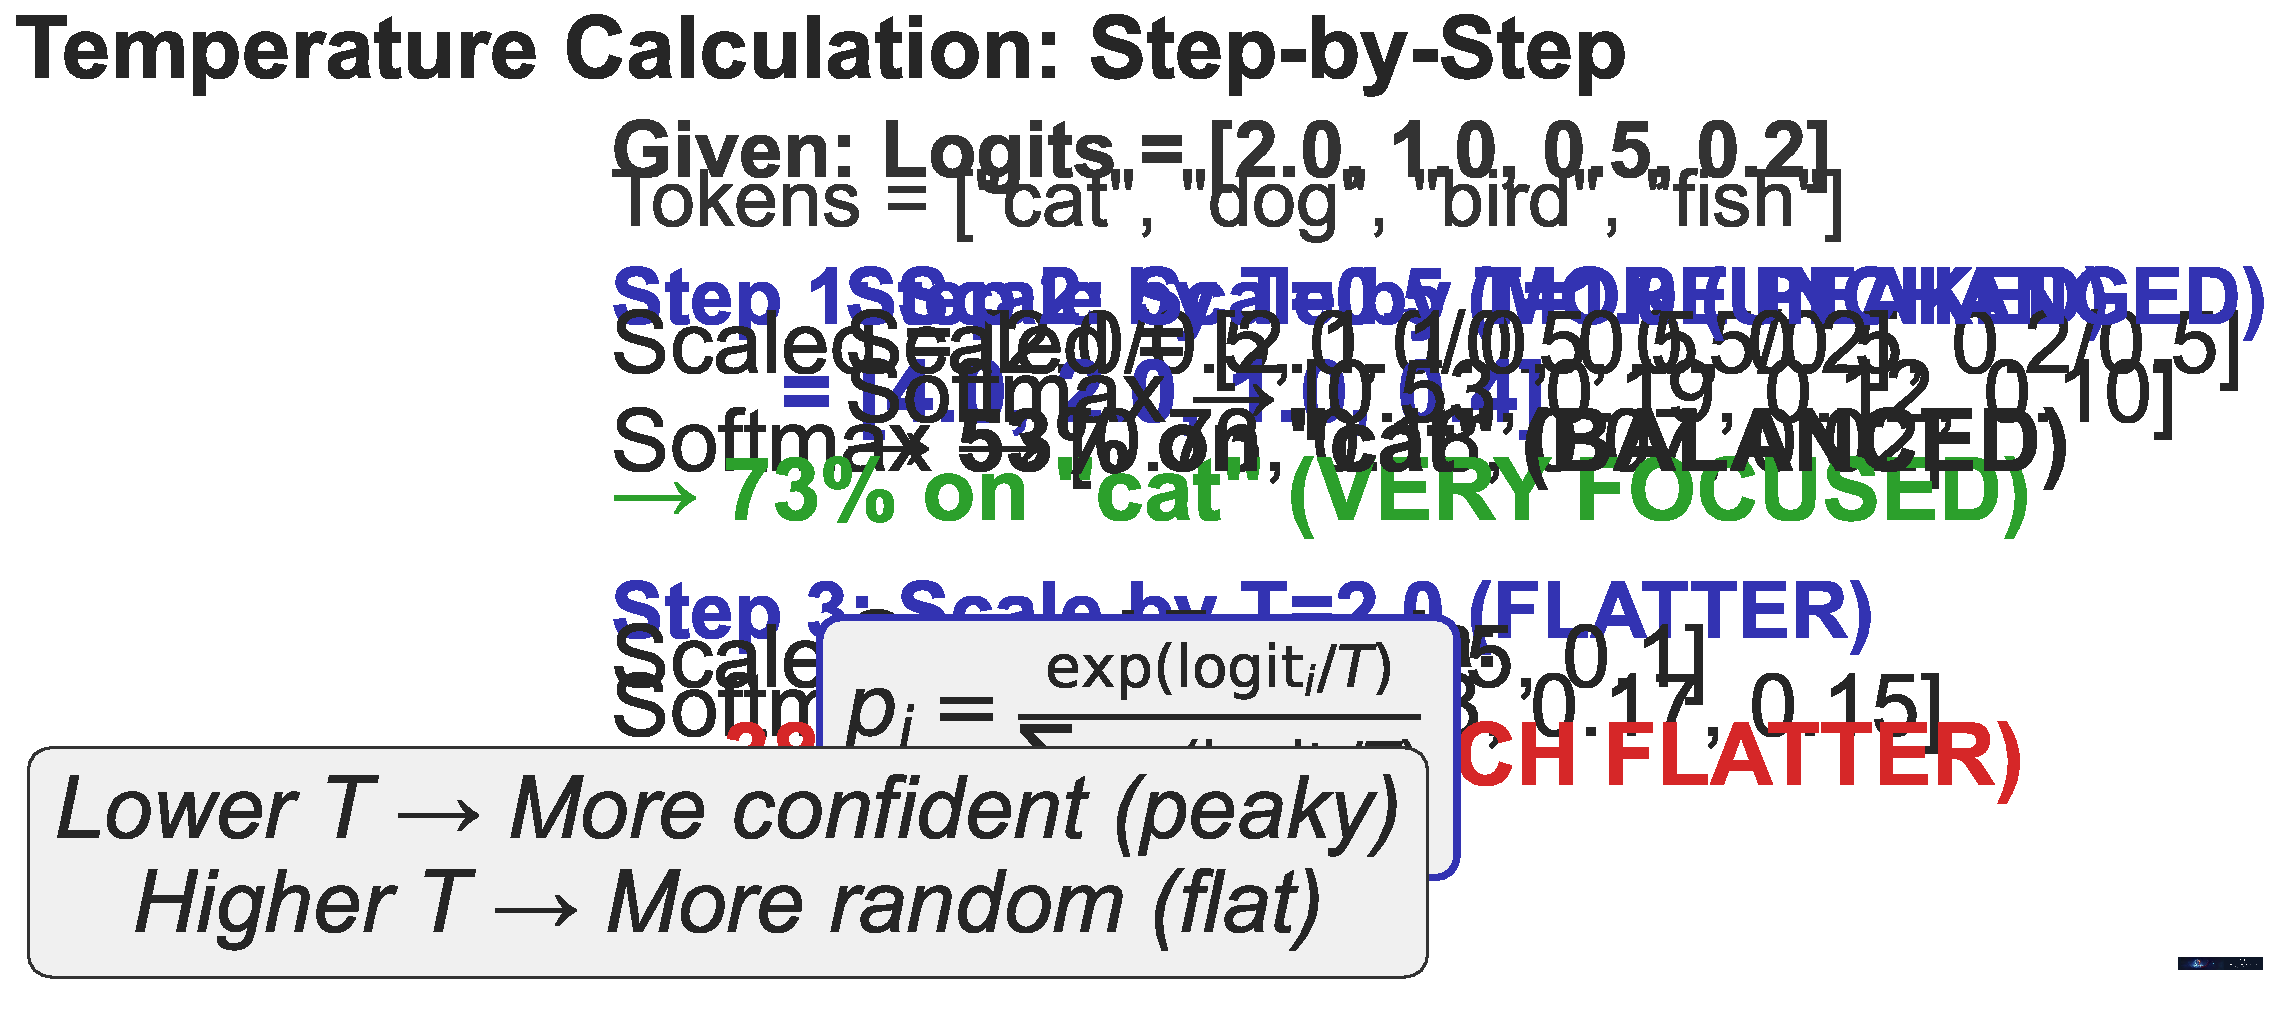
\includegraphics[width=0.70\textwidth]{../figures/temperature_calculation_bsc.pdf}
\end{center}
\bottomnote{Concrete numbers show how temperature scaling works}
\end{frame}

\begin{frame}[t]{Temperature: Detail}
\small
\begin{columns}[T]
\column{0.49\textwidth}
\textbf{How It Works}:

Given logits $z_1, ..., z_V$

\vspace{2mm}
Scale by temperature $T$:

$$p_i = \frac{\exp(z_i / T)}{\sum_j \exp(z_j / T)}$$

Sample from $p$

\vspace{2mm}
\textbf{Effect}:

$T \rightarrow 0$: argmax

$T = 1$: standard softmax

$T \rightarrow \infty$: uniform

\column{0.49\textwidth}
\textbf{Practical Settings}:

\begin{itemize}
\item \textbf{T = 0.1-0.3}: Factual Q\&A
\item \textbf{T = 0.7}: Chatbots
\item \textbf{T = 0.9-1.2}: Creative
\item \textbf{T = 1.5+}: Experimental
\end{itemize}

\vspace{2mm}
\colorbox{mllavender4}{\parbox{0.90\textwidth}{
+ Simple to implement

+ Continuous control

- No quality guarantee

- Can be nonsense
}}

\end{columns}
\bottomnote{Temperature: simplest randomness control}
\end{frame}

\begin{frame}[t]{Top-k Sampling: Filter the Tail}
\vspace{-0.3cm}
\begin{center}
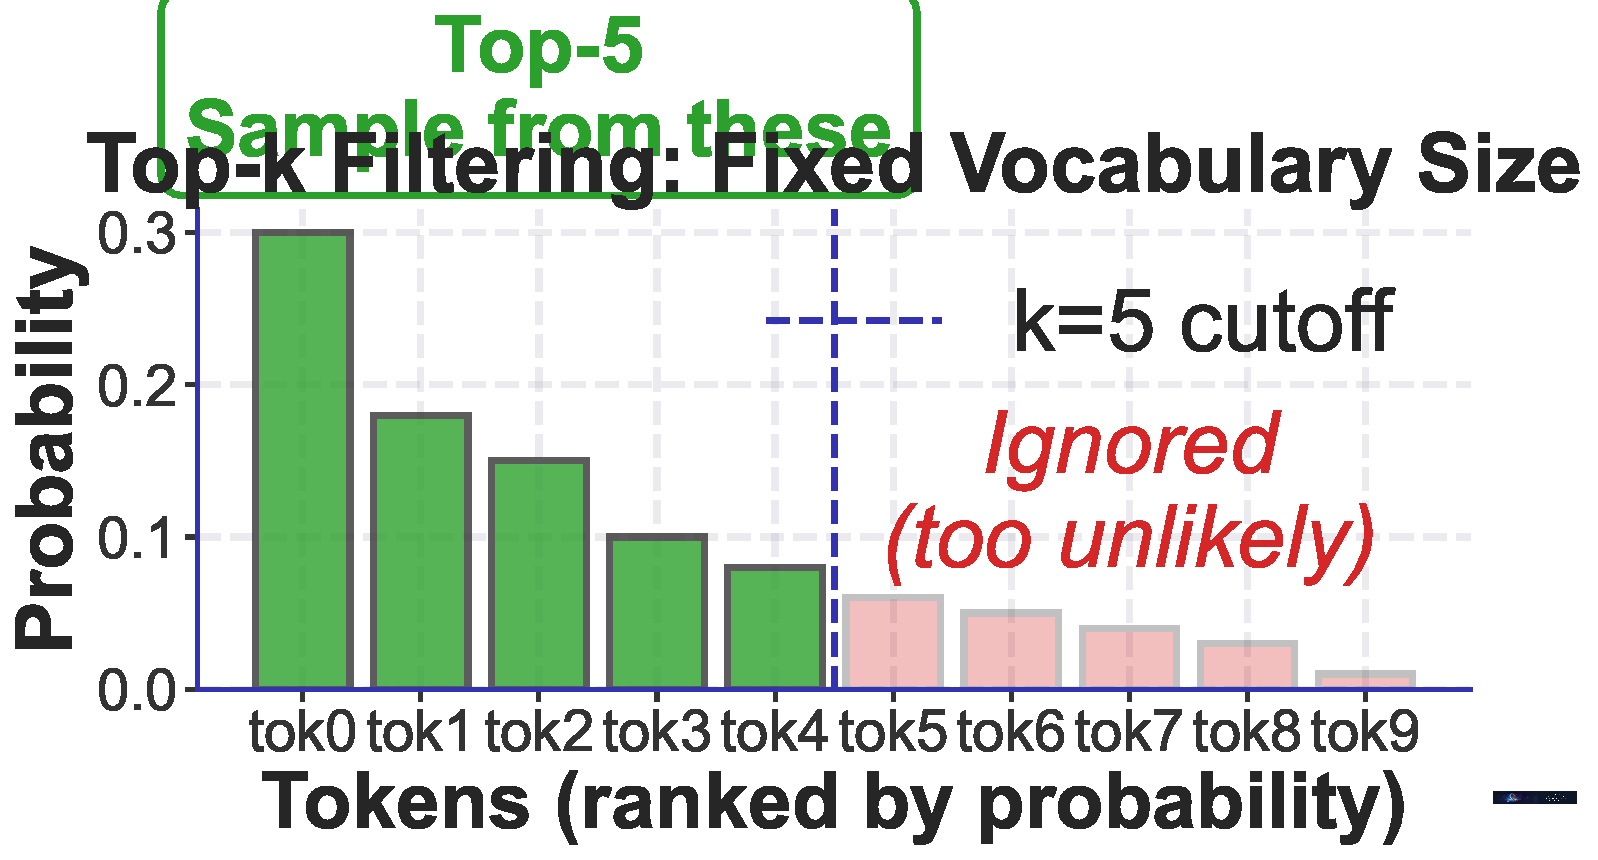
\includegraphics[width=0.70\textwidth]{../figures/topk_filtering_bsc.pdf}
\end{center}
\begin{center}
\colorbox{mllavender3}{\parbox{0.75\textwidth}{
\centering
\textcolor{mlpurple}{\textbf{Key Insight}}: Only sample from top-k most likely tokens
}}
\end{center}
\bottomnote{Prevents sampling from long tail of unlikely words}
\end{frame}

\begin{frame}[t]{Top-k: Worked Example (k=3)}
\vspace{-0.3cm}
\begin{center}
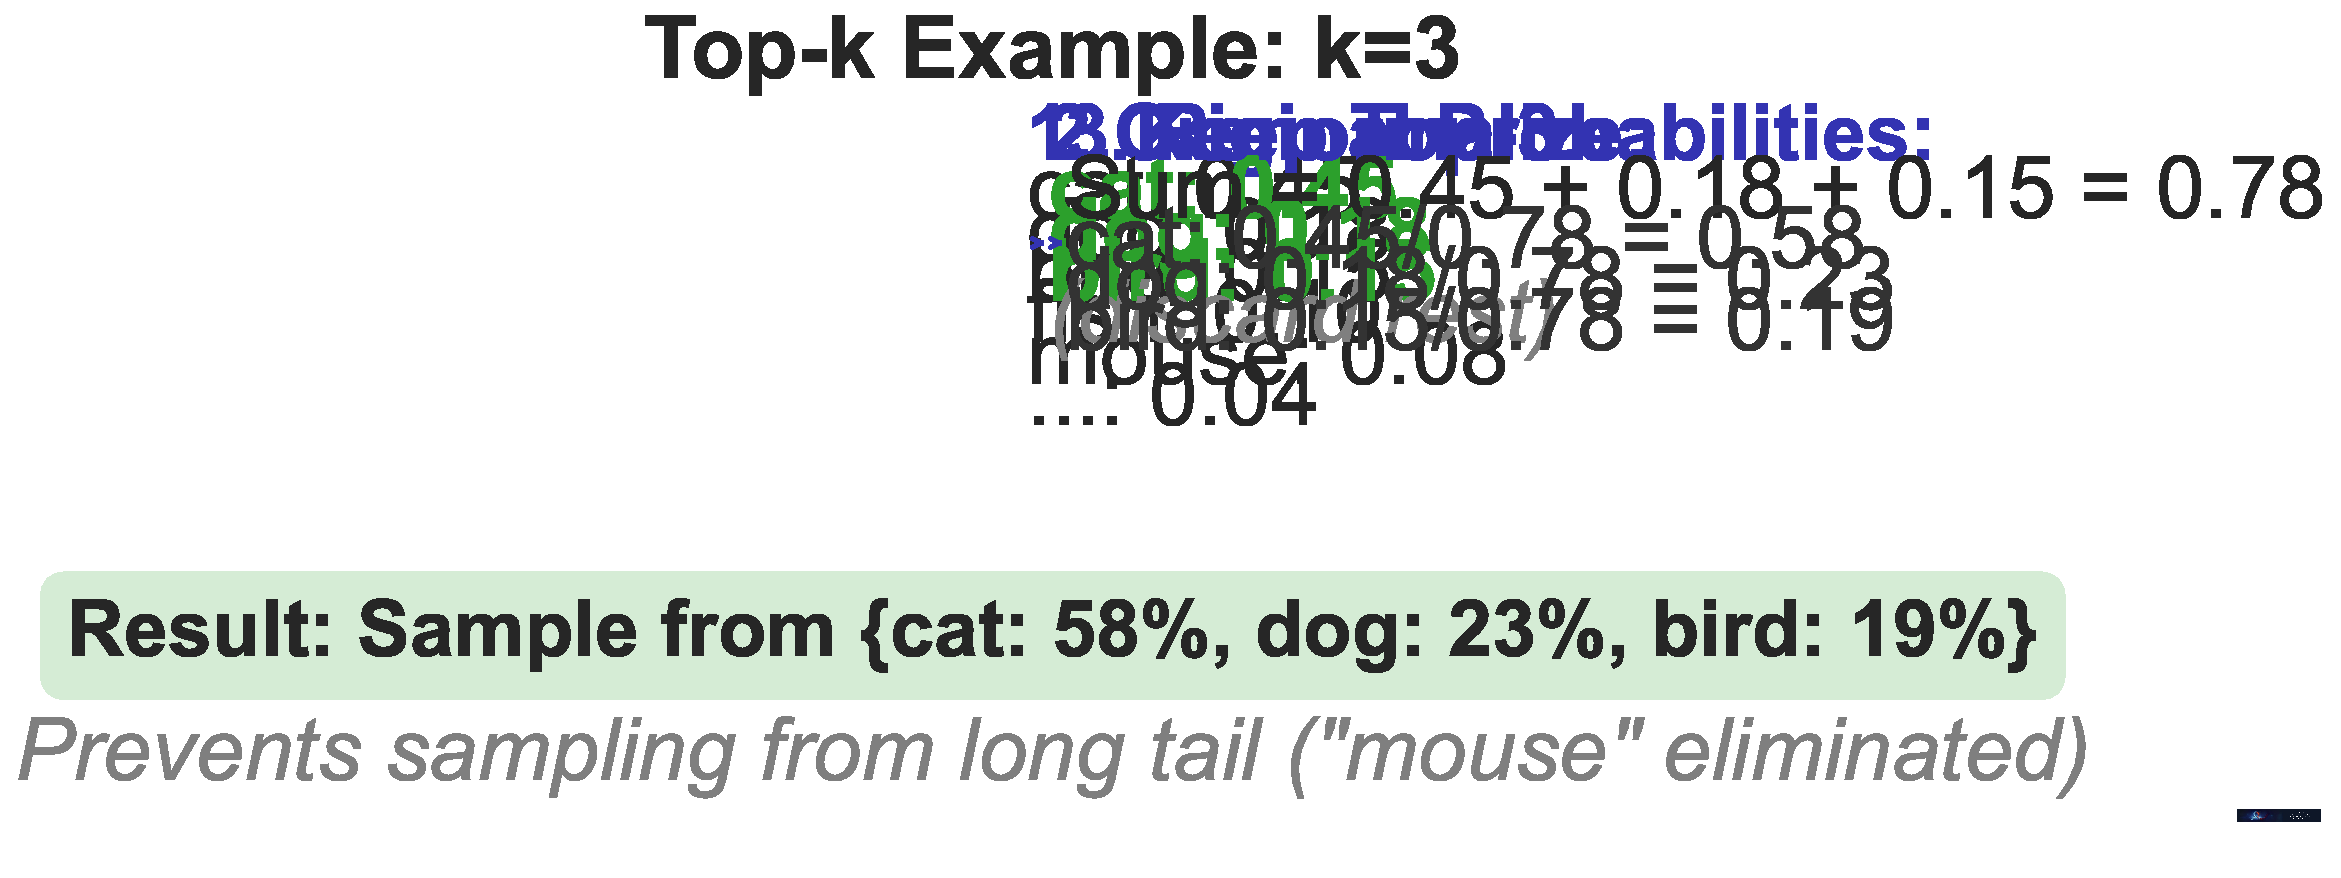
\includegraphics[width=0.70\textwidth]{../figures/topk_example_bsc.pdf}
\end{center}
\bottomnote{Filtering + renormalization prevents tail sampling}
\end{frame}

\begin{frame}[t]{Top-k: Detail}
\small
\begin{columns}[T]
\column{0.49\textwidth}
\textbf{Algorithm}:

\begin{enumerate}
\item Compute $P(w_i)$ for all
\item Sort by probability
\item Keep only top-k
\item Renormalize
\item Sample from $p'$
\end{enumerate}

\vspace{2mm}
\textbf{Example} (k=3):

Original: [0.45, 0.18, 0.15, ...]

Keep: [0.45, 0.18, 0.15]

Renorm: [0.58, 0.23, 0.19]

\column{0.49\textwidth}
\textbf{Typical Values}:

k = 40-50 (balanced)

k = 10-20 (focused)

k = 100+ (very diverse)

\vspace{2mm}
\colorbox{mlred!20}{\parbox{0.90\textwidth}{
\textbf{Limitation}:

Fixed cutoff regardless of distribution!

Peaked: Wastes mass

Flat: Too many bad tokens
}}

\vspace{2mm}
\textbf{Solution}: Dynamic cutoff

\end{columns}
\bottomnote{Top-k improves over temperature but inflexible}
\end{frame}

\begin{frame}[t]{Nucleus (Top-p) Sampling: Dynamic Cutoff}
\vspace{-0.3cm}
\begin{center}
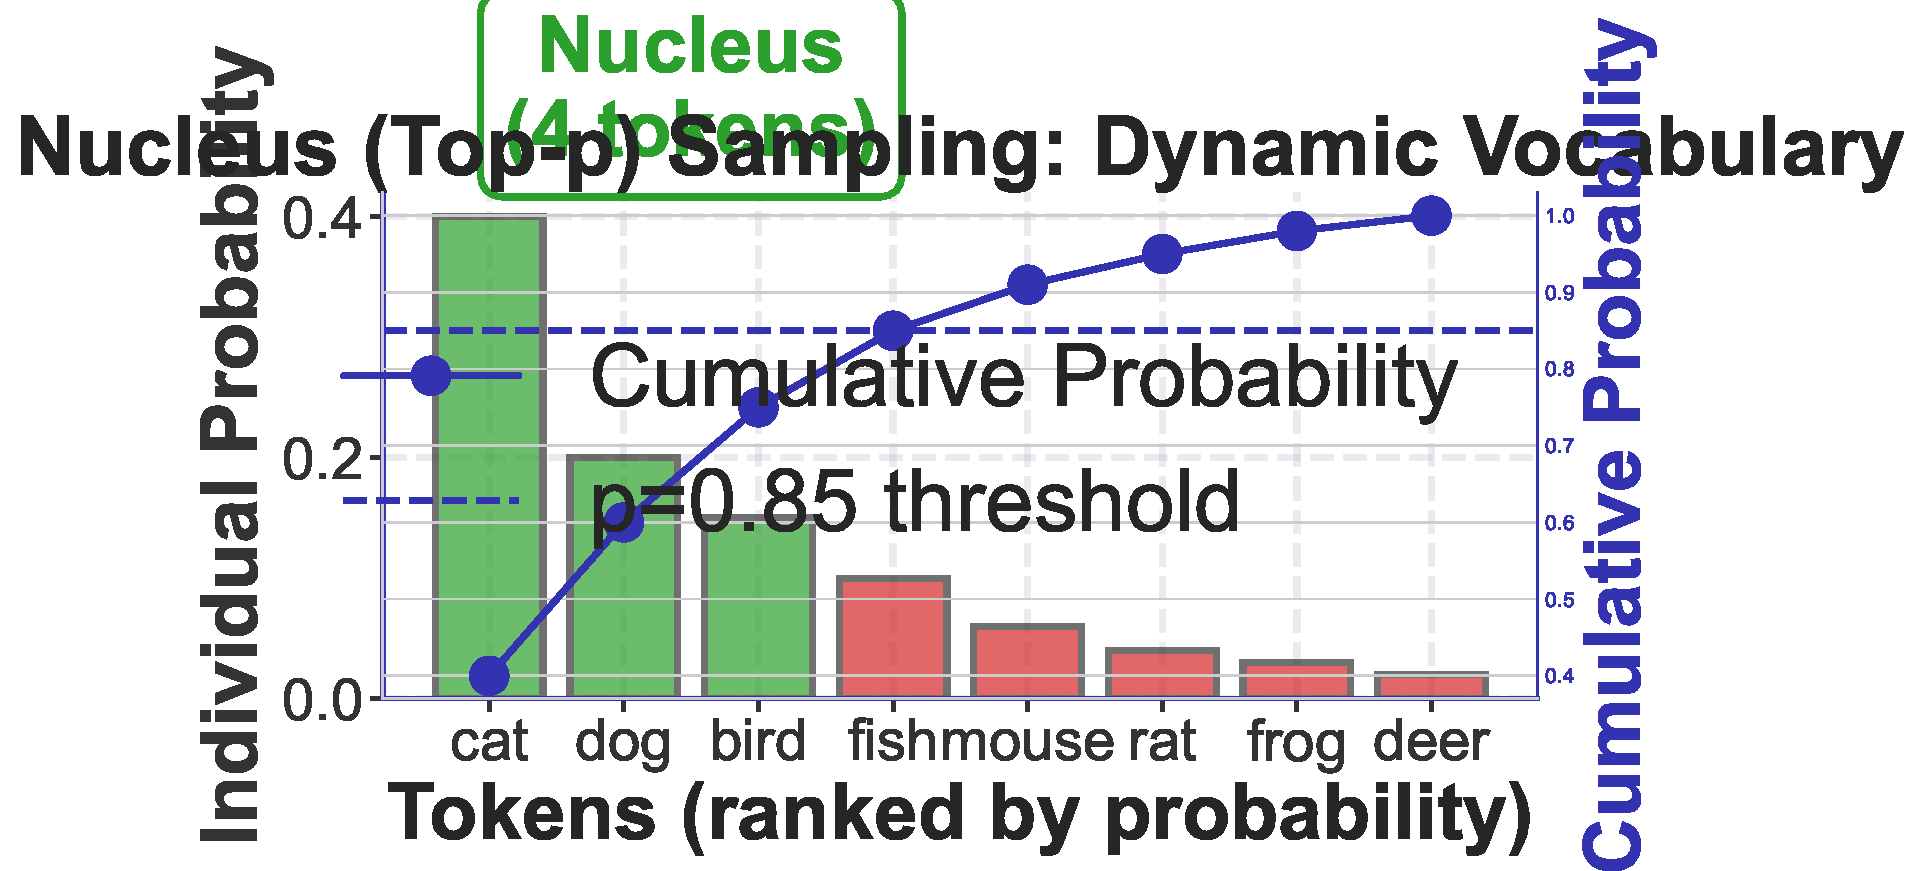
\includegraphics[width=0.70\textwidth]{../figures/nucleus_process_bsc.pdf}
\end{center}
\begin{center}
\colorbox{mllavender3}{\parbox{0.75\textwidth}{
\centering
\textcolor{mlpurple}{\textbf{Key Insight}}: Adapt vocabulary size to distribution shape
}}
\end{center}
\bottomnote{Nucleus size grows/shrinks based on probability spread}
\end{frame}

\begin{frame}[t]{Nucleus: How Distribution Shape Matters}
\vspace{-0.3cm}
\begin{center}
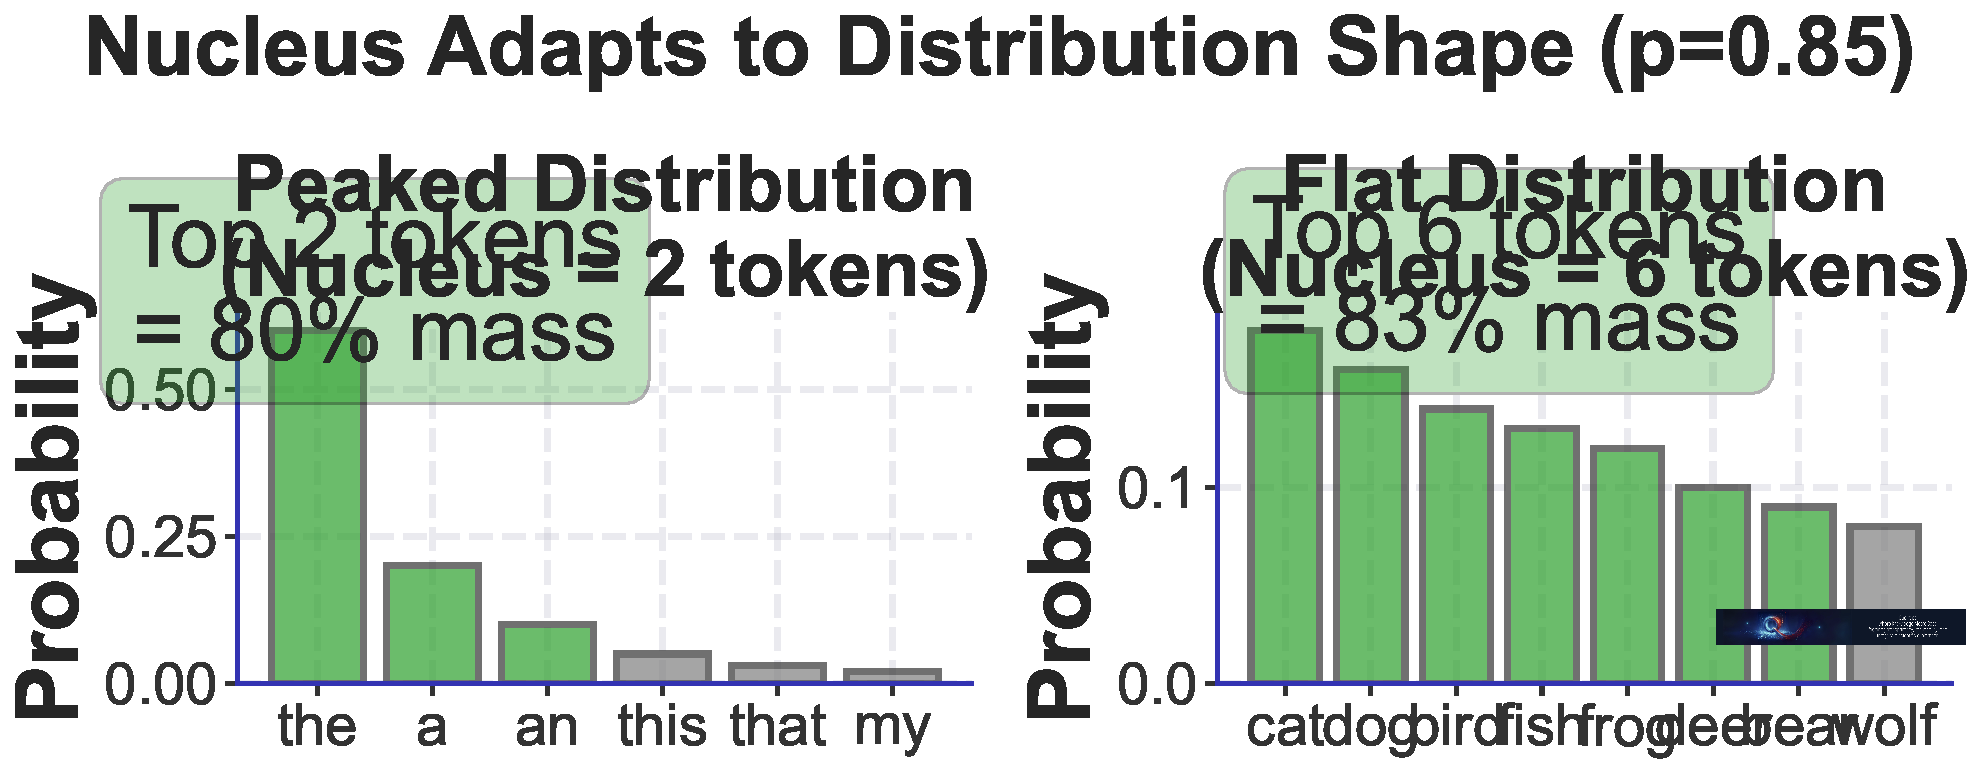
\includegraphics[width=0.70\textwidth]{../figures/nucleus_cumulative_bsc.pdf}
\end{center}
\bottomnote{Same p value → different vocabulary for peaked vs flat}
\end{frame}

\begin{frame}[t]{Nucleus (Top-p): Detail}
\small
\begin{columns}[T]
\column{0.49\textwidth}
\textbf{Algorithm}:

\begin{enumerate}
\item Sort tokens by $P(w_i)$
\item Compute cumulative sum
\item Find smallest set where $\text{cum} \geq p$
\item Sample from nucleus
\end{enumerate}

\vspace{2mm}
\textbf{Example} (p=0.85):

Cumsum: [0.40, 0.60, 0.75, 0.85]

Nucleus: First 4 tokens

\column{0.49\textwidth}
\textbf{Recommended}:

\begin{itemize}
\item p = 0.85-0.90: Dialogue
\item p = 0.90-0.95: Creative
\item p = 0.95-0.99: Very diverse
\end{itemize}

\vspace{2mm}
\colorbox{mlgreen!20}{\parbox{0.90\textwidth}{
\textbf{Why Better}:

Peaked → small nucleus

Flat → large nucleus

Adapts automatically!
}}

\vspace{2mm}
\textbf{Current Standard}

ChatGPT, Claude, GPT-4

\end{columns}
\bottomnote{Nucleus: modern standard for high-quality generation}
\end{frame}

% === CONTRASTIVE SEARCH (3 SLIDES) ===

\begin{frame}[t]{The Degeneration Problem}
\vspace{-0.3cm}
\begin{center}
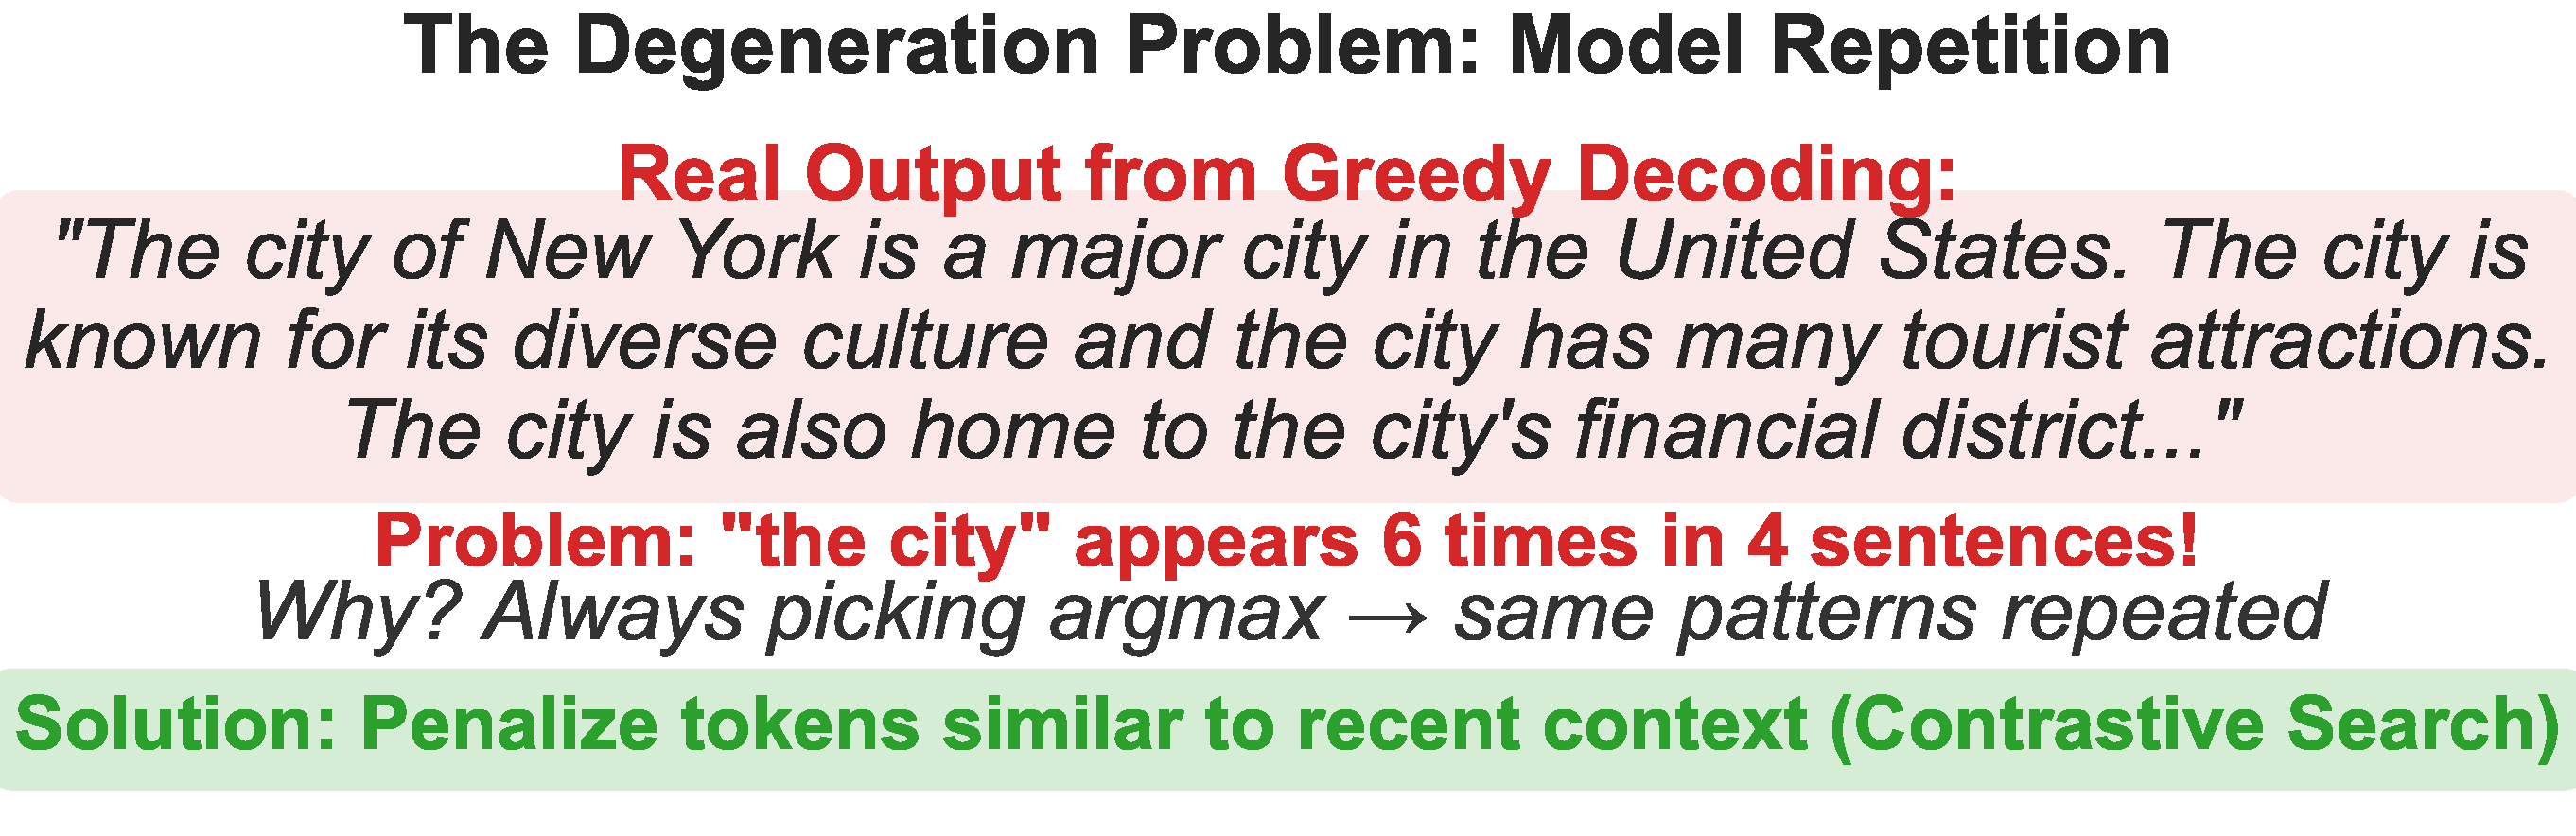
\includegraphics[width=0.70\textwidth]{../figures/degeneration_problem_bsc.pdf}
\end{center}
\begin{center}
\colorbox{mllavender3}{\parbox{0.75\textwidth}{
\centering
\textcolor{mlpurple}{\textbf{Discovery}}: Why do models repeat themselves?
}}
\end{center}
\bottomnote{Greedy/beam maximize probability - but high prob = repeating recent context}
\end{frame}

\begin{frame}[t]{Contrastive Search: Penalize Repetition (2025)}
\vspace{-0.3cm}
\begin{center}
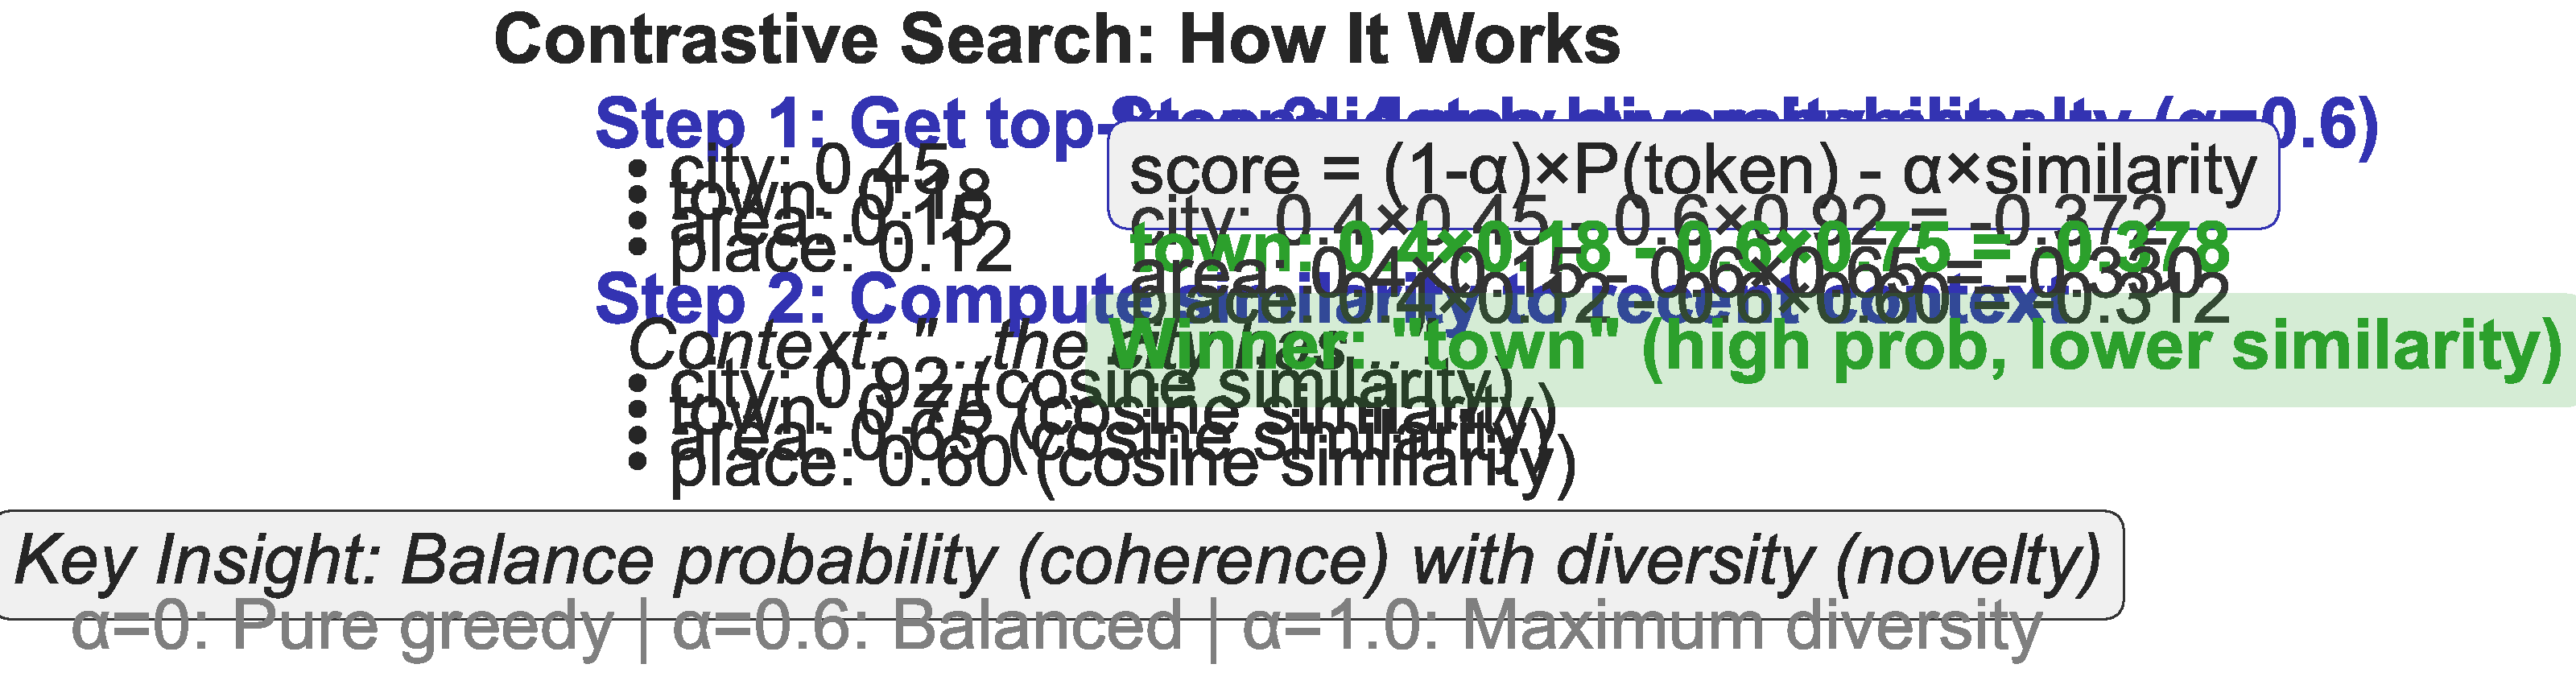
\includegraphics[width=0.70\textwidth]{../figures/contrastive_mechanism_bsc.pdf}
\end{center}
\begin{center}
\colorbox{mllavender3}{\parbox{0.75\textwidth}{
\centering
\textcolor{mlpurple}{\textbf{Key Insight}}: Balance probability with diversity penalty
}}
\end{center}
\bottomnote{Explicitly avoid copying recent context - prevents degeneration}
\end{frame}

\begin{frame}[t]{Contrastive vs Nucleus: Comparison}
\vspace{-0.3cm}
\begin{center}
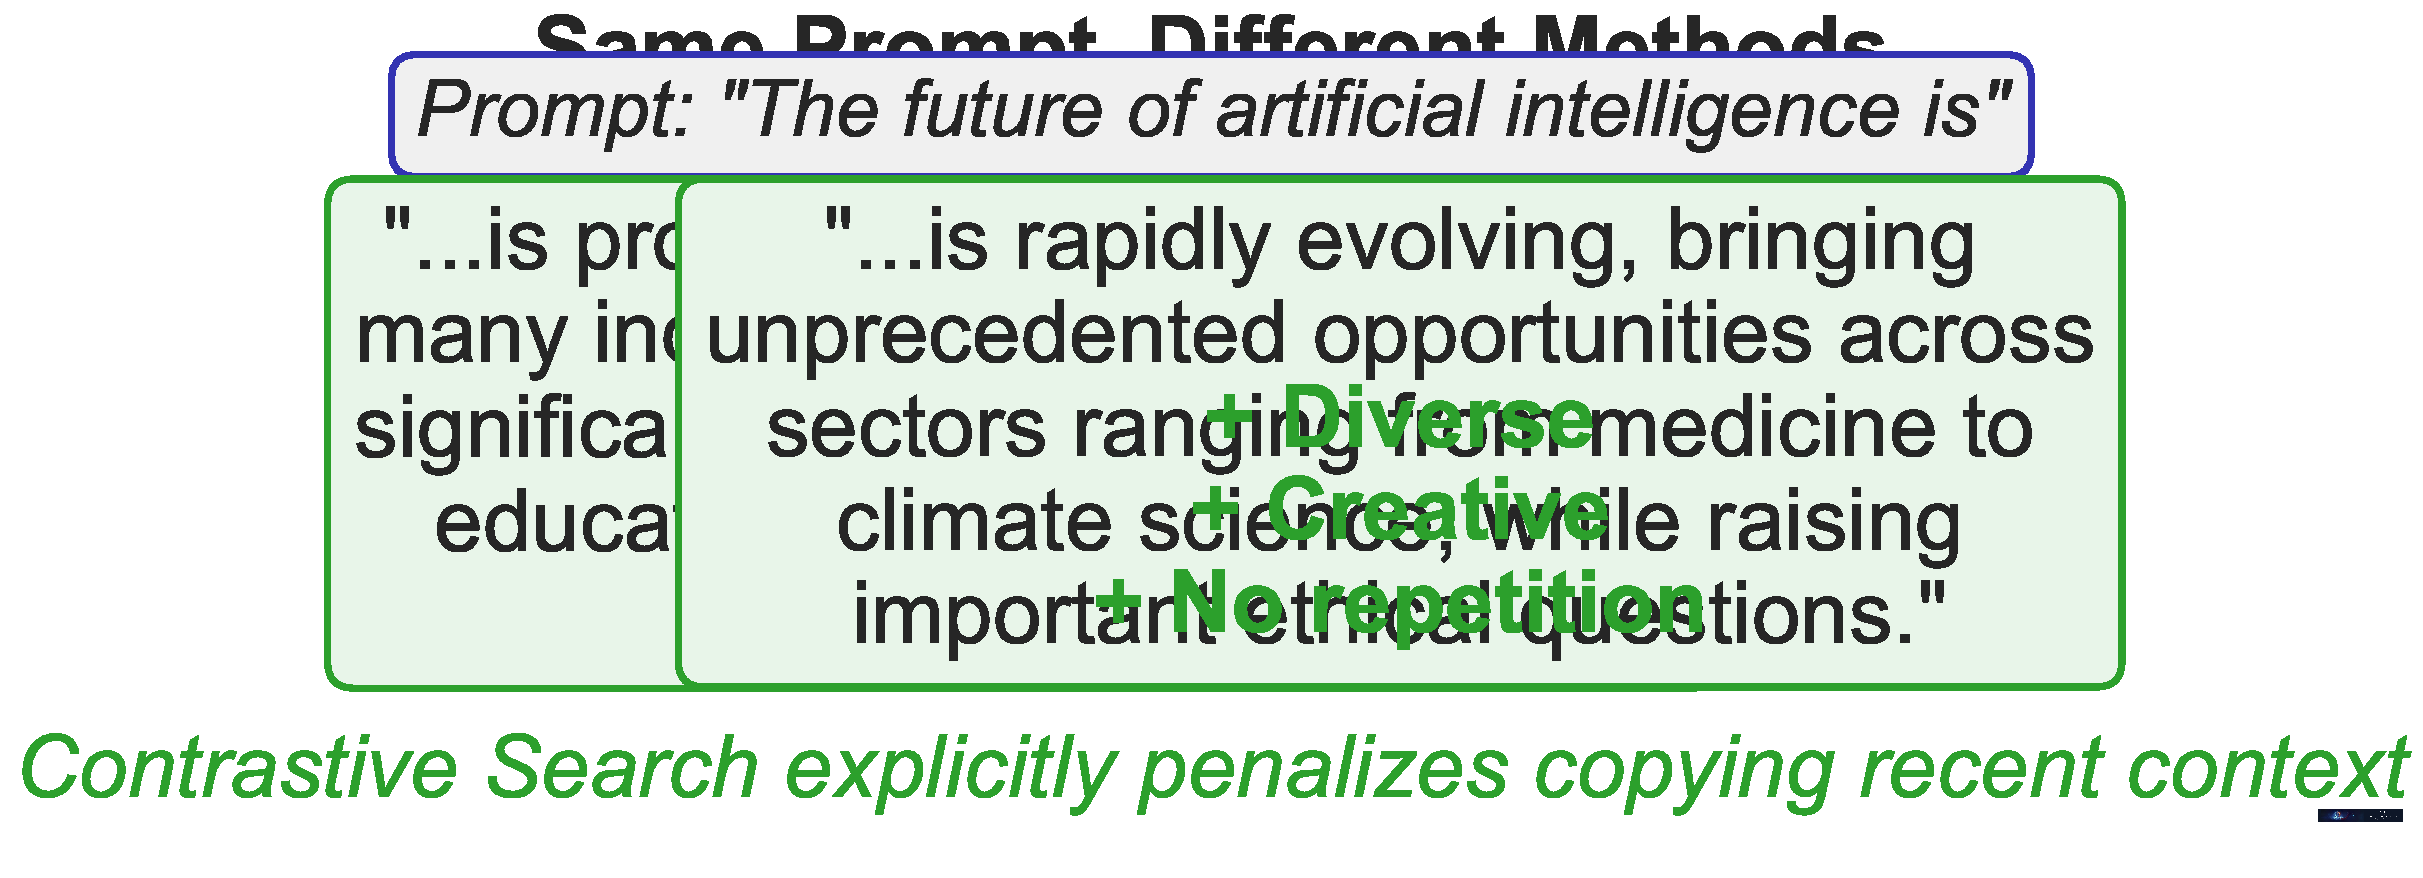
\includegraphics[width=0.75\textwidth]{../figures/contrastive_vs_nucleus_bsc.pdf}
\end{center}
\bottomnote{Contrastive prevents repetition better for long generation}
\end{frame}

% === QUALITY-DIVERSITY OPTIMIZATION (1 SLIDE) ===

\begin{frame}[t]{All Methods on Quality-Diversity Space}
\vspace{-0.3cm}
\begin{center}
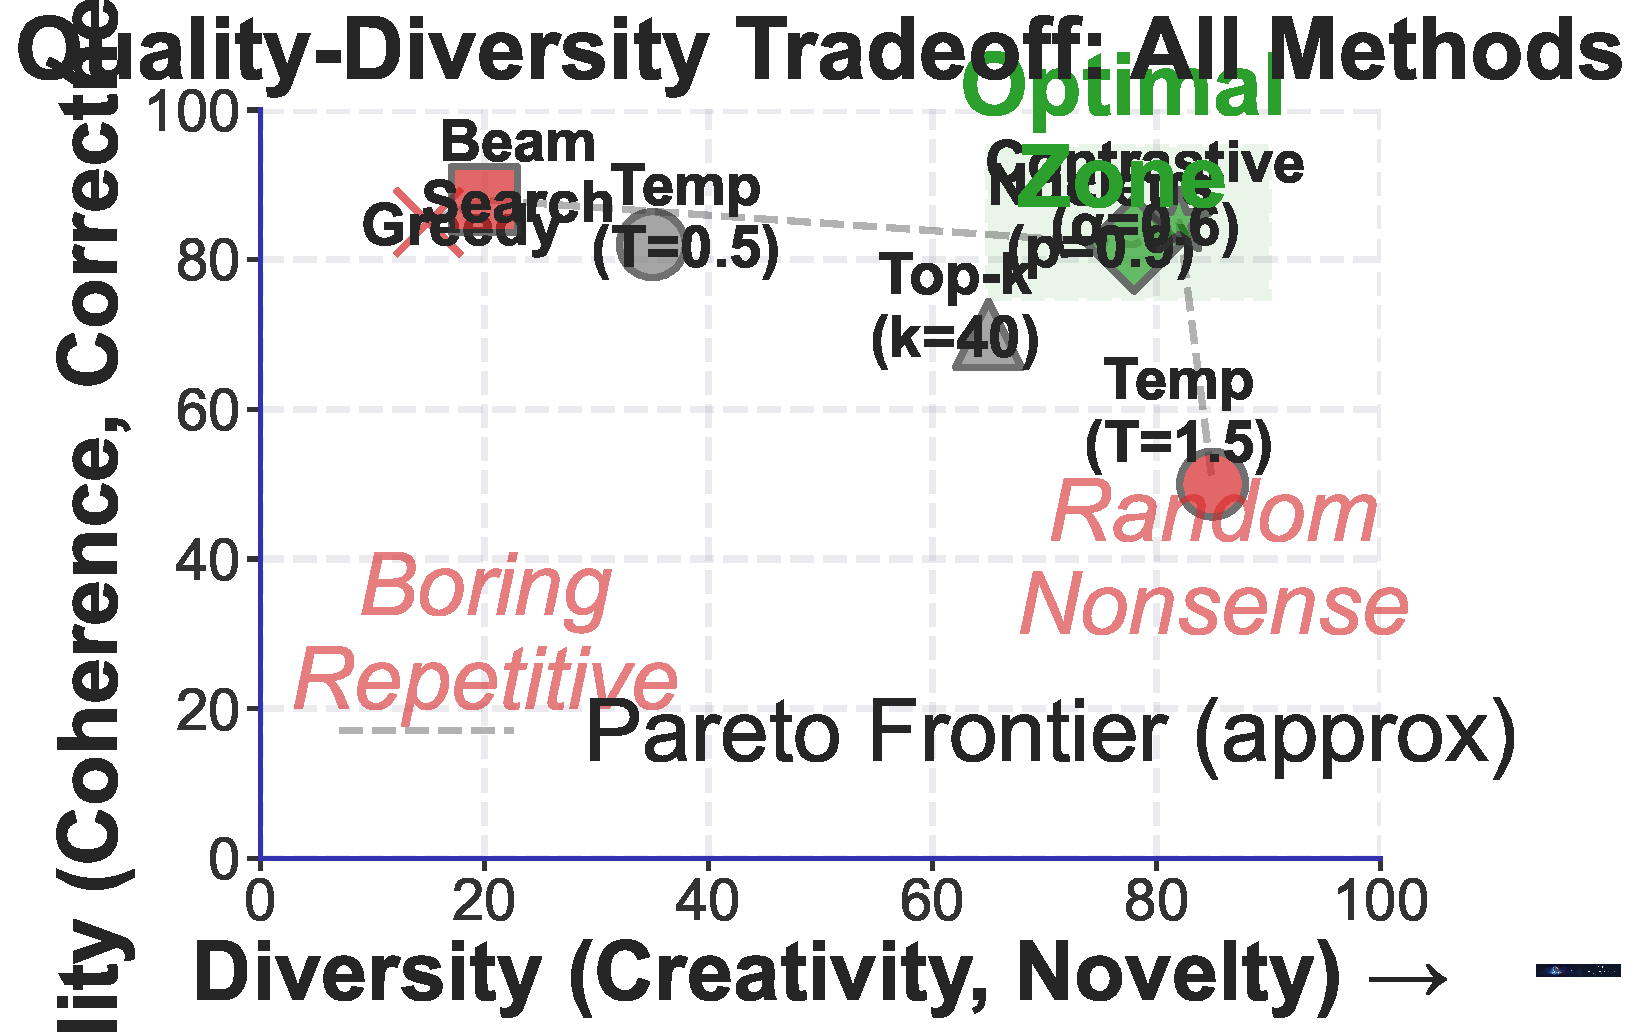
\includegraphics[width=0.70\textwidth]{../figures/quality_diversity_pareto_bsc.pdf}
\end{center}
\begin{center}
\colorbox{mllavender3}{\parbox{0.75\textwidth}{
\centering
\textcolor{mlpurple}{\textbf{Pareto Frontier}}: No method dominates all others
}}
\end{center}
\bottomnote{Choose based on task: deterministic (left), creative (right)}
\end{frame}

% === TASK-SPECIFIC RECOMMENDATIONS (3 SLIDES) ===

\begin{frame}[t]{Choosing the Right Method: Decision Tree}
\vspace{-0.3cm}
\begin{center}
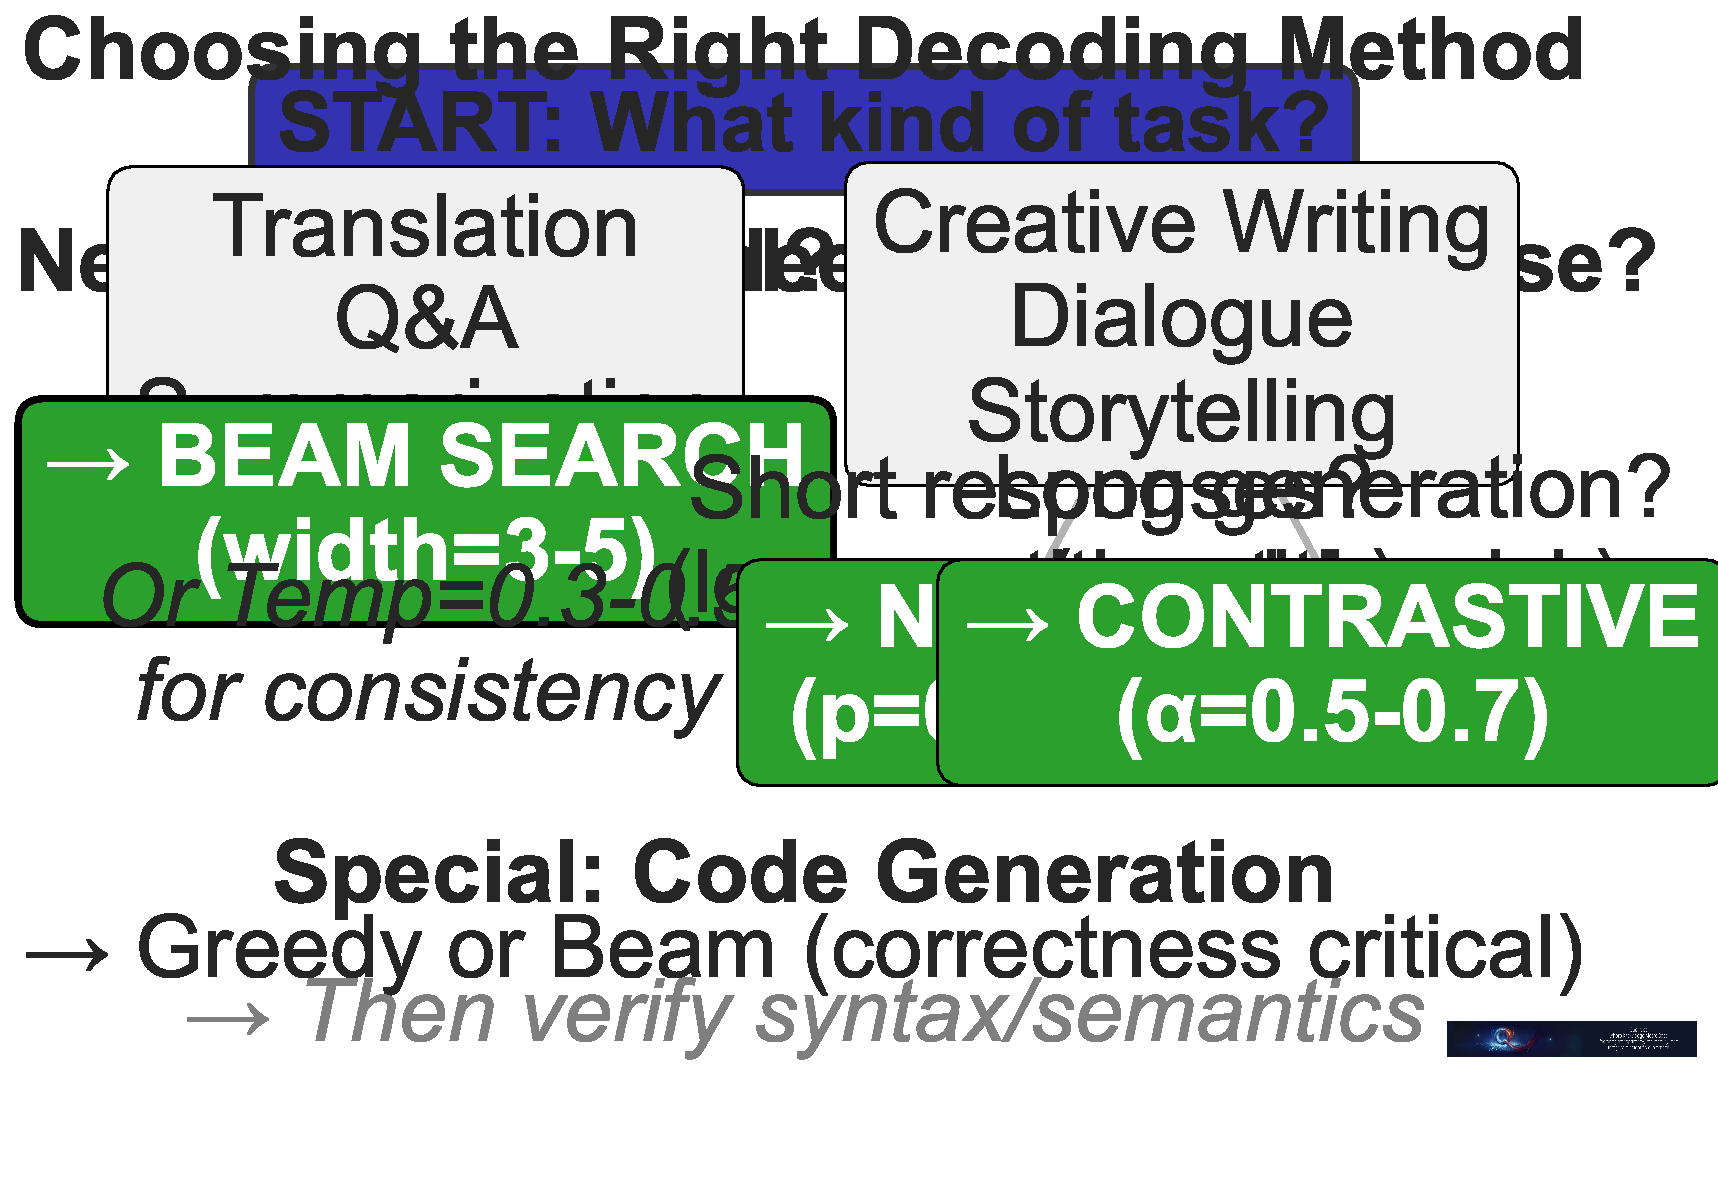
\includegraphics[width=0.70\textwidth]{../figures/task_method_decision_tree_bsc.pdf}
\end{center}
\bottomnote{Start with task requirements, follow tree to recommended method}
\end{frame}

\begin{frame}[t]{Task-Specific Recommendations (2025)}
\vspace{-0.3cm}
\begin{center}
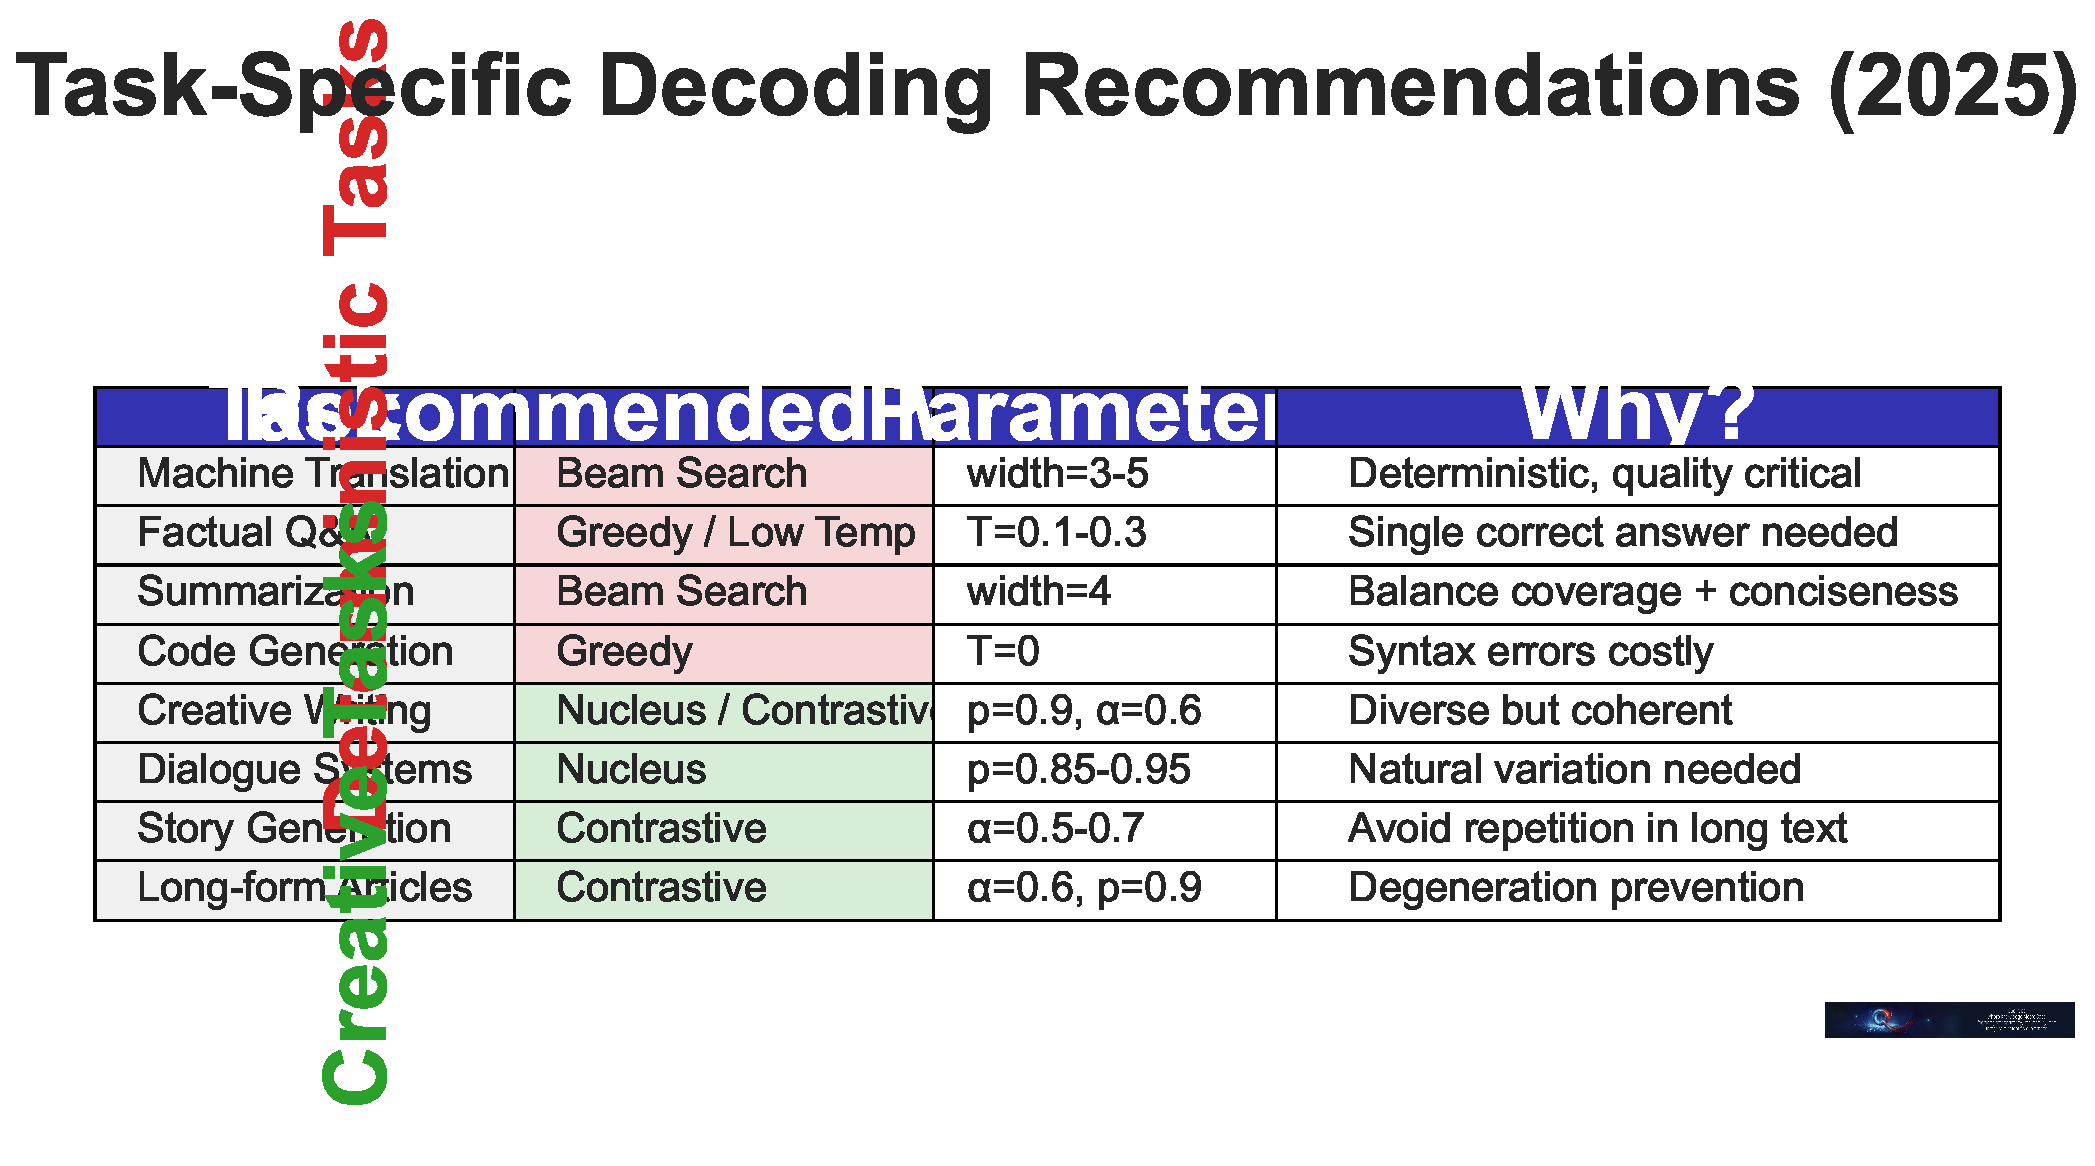
\includegraphics[width=0.75\textwidth]{../figures/task_recommendations_table_bsc.pdf}
\end{center}
\bottomnote{Comprehensive mapping: 8 tasks → optimal strategies}
\end{frame}

\begin{frame}[t]{Computational Costs Matter}
\vspace{-0.3cm}
\begin{center}
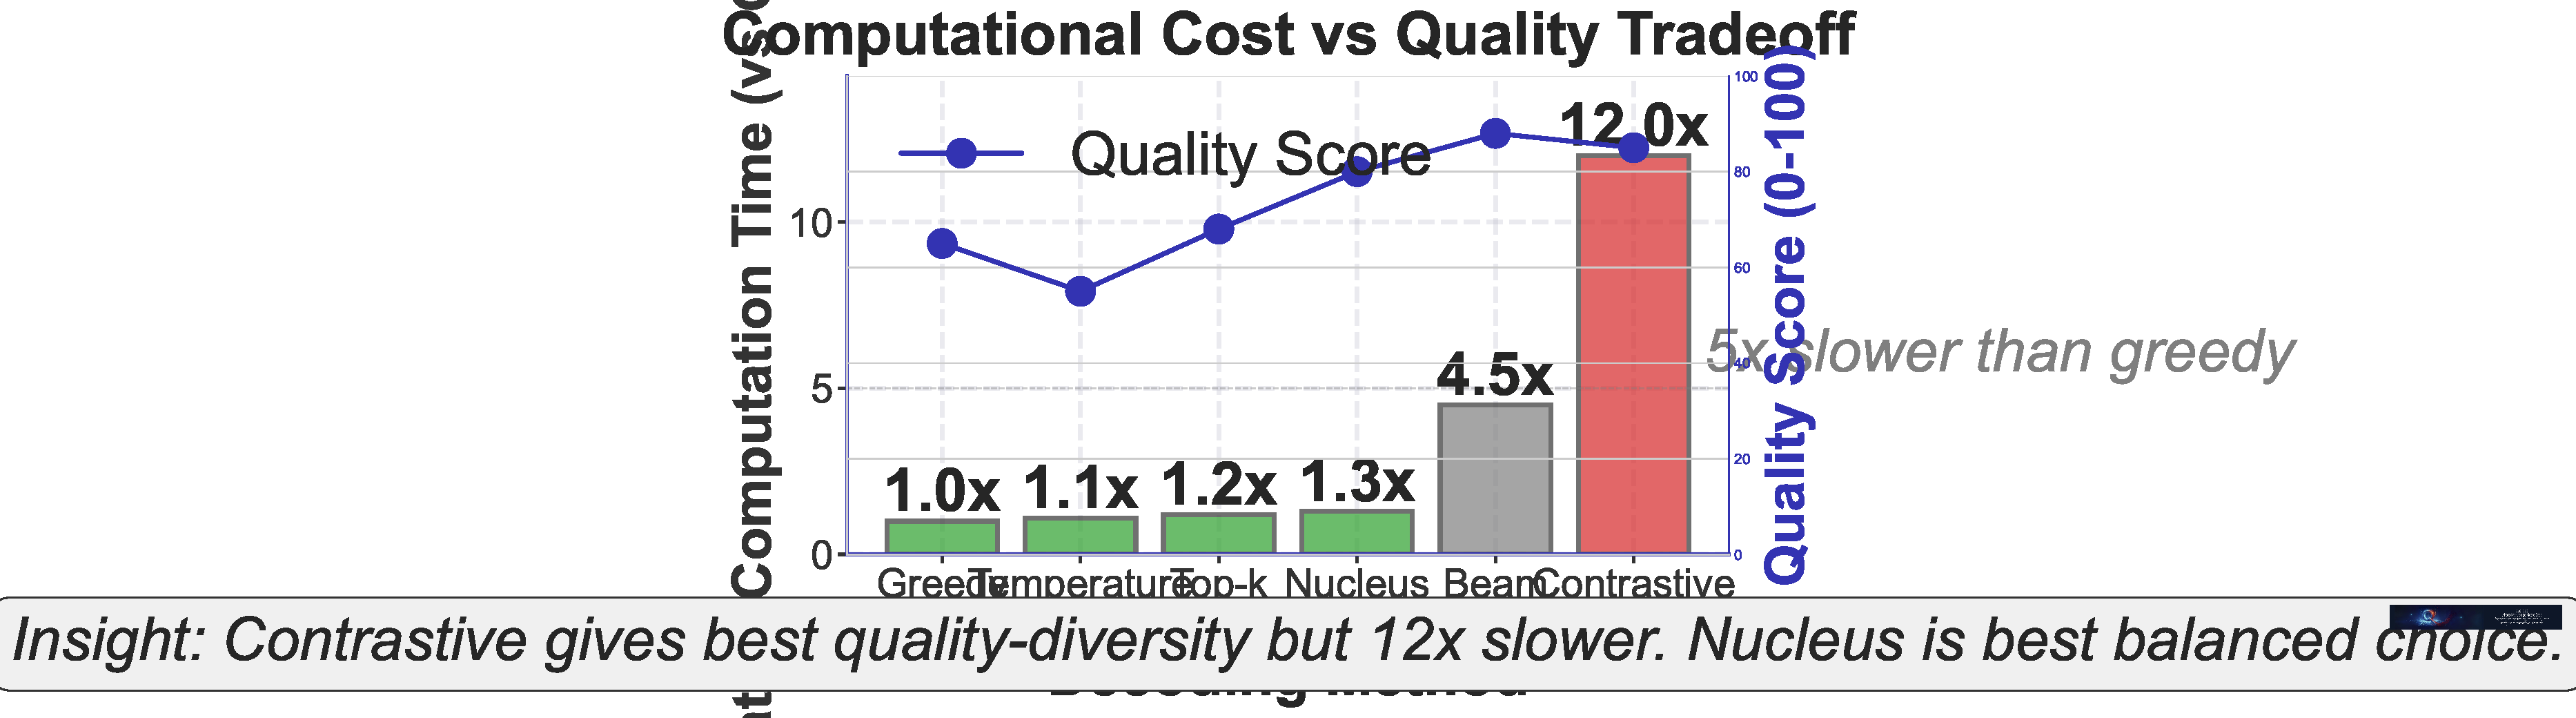
\includegraphics[width=0.70\textwidth]{../figures/computational_cost_comparison_bsc.pdf}
\end{center}
\begin{center}
\colorbox{mllavender3}{\parbox{0.75\textwidth}{
\centering
Contrastive: best quality-diversity but 12× slower. \textcolor{mlgreen}{\textbf{Nucleus: best balanced}}
}}
\end{center}
\bottomnote{Production tradeoff: Quality vs speed vs diversity}
\end{frame}

% === SUMMARY (2 SLIDES) ===

\begin{frame}[t]{Key Takeaways}
\begin{enumerate}
\item \textcolor{mlpurple}{\textbf{Deterministic}} (Greedy, Beam): High quality, no diversity → factual tasks
\item \textcolor{mlpurple}{\textbf{Temperature}}: Simple randomness control → universal but crude
\item \textcolor{mlpurple}{\textbf{Top-k}}: Fixed vocabulary filter → prevents tail sampling
\item \textcolor{mlpurple}{\textbf{Nucleus (Top-p)}}: Dynamic cutoff → modern standard, adapts
\item \textcolor{mlpurple}{\textbf{Contrastive (NEW)}}: Degeneration prevention → long creative text
\item \textcolor{mlpurple}{\textbf{Task matters}}: Translation → Beam | Dialogue → Nucleus | Stories → Contrastive
\end{enumerate}

\vspace{3mm}
\begin{center}
\colorbox{mllavender2}{\parbox{0.85\textwidth}{
\centering
\textbf{Next}: Lab - Implement all 6 methods, measure quality-diversity tradeoffs
}}
\end{center}

\bottomnote{Decoding strategy matters as much as model architecture}
\end{frame}

% ============================================
% TECHNICAL APPENDIX (19 SLIDES)
% ============================================

\begin{frame}[t]{}
\begin{center}
\Huge\textcolor{mlpurple}{\textbf{Technical Appendix}}

\vspace{1cm}
\large 19 slides: Complete mathematical treatment

\vspace{0.5cm}
\textcolor{mlgray}{A1-A5: Beam Search Mathematics}

\textcolor{mlgray}{A6-A10: Sampling Mathematics}

\textcolor{mlgray}{A11-A14: Contrastive Search \& Degeneration}

\textcolor{mlgray}{A15-A19: Advanced Topics \& Production}
\end{center}
\end{frame}

% === A1-A5: BEAM SEARCH MATHEMATICS ===

\begin{frame}[t]{A1: Beam Search Formulation}
\small
\textbf{Objective}: Find $y^* = \argmax P(y | x)$

\vspace{2mm}
\textbf{Decomposition}:

$$P(y | x) = \prod_{t=1}^T P(y_t | y_{<t}, x)$$

\textbf{Log-probability}:

$$\log P(y | x) = \sum_{t=1}^T \log P(y_t | y_{<t}, x)$$

\vspace{2mm}
\textbf{Beam Search Approximation}:

Instead of $V^T$ sequences, maintain top-k hypotheses

\vspace{2mm}
\colorbox{mllavender4}{\parbox{0.85\textwidth}{
\textbf{Complexity}:

Time: $O(k \cdot V \cdot T)$

Space: $O(k \cdot T)$
}}

\bottomnote{Tractable approximation to exact search}
\end{frame}

\begin{frame}[t]{A2: Length Normalization}
\vspace{-0.3cm}
\begin{center}
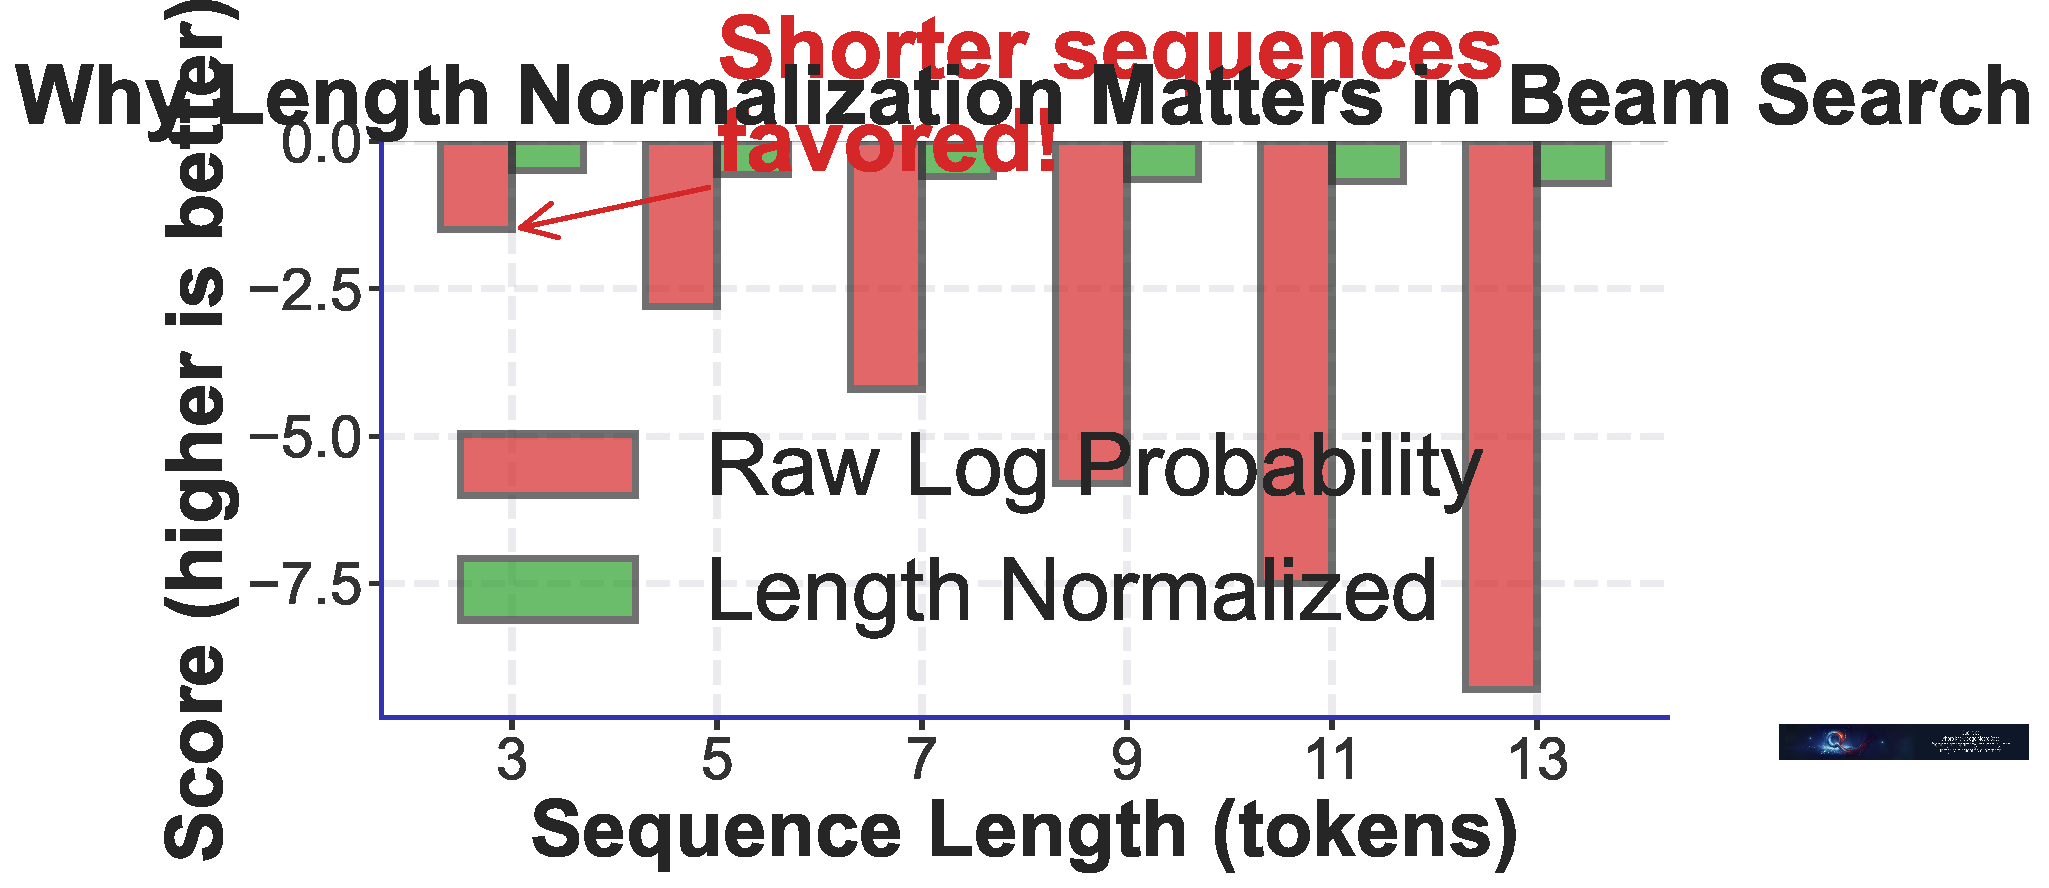
\includegraphics[width=0.60\textwidth]{../figures/length_normalization_bsc.pdf}
\end{center}

\vspace{2mm}
\small
\textbf{Solution}: Normalize by length

$$\text{score}(y) = \frac{1}{|y|^\alpha} \log P(y) \quad \text{where } \alpha \in [0.5, 1.0]$$

\bottomnote{Length normalization essential for fair comparison}
\end{frame}

\begin{frame}[t]{A3: Beam Search Variants}
\small
\begin{columns}[T]
\column{0.49\textwidth}
\textbf{Diverse Beam}:

Partition beams into groups

Penalize within-group similarity

\vspace{2mm}
\textbf{Constrained Beam}:

Force certain tokens

Keywords, entities

\column{0.49\textwidth}
\textbf{Stochastic Beam}:

Sample beams (not argmax)

More diverse

\vspace{2mm}
\textbf{Block n-gram}:

Penalize n-gram repetition

``city is a city'' prevention
\end{columns}
\bottomnote{Many variants for specific requirements}
\end{frame}

\begin{frame}[t]{A4: Beam Search Stopping}
\small
\textbf{When to stop}?

\vspace{3mm}
\begin{enumerate}
\item \textbf{Fixed length}: Stop at $T_{\max}$ (simple but rigid)
\item \textbf{END token}: Special token (most common)
\item \textbf{Score threshold}: When best cannot improve
\item \textbf{Timeout}: Computational budget
\end{enumerate}

\bottomnote{Stopping criterion affects output length}
\end{frame}

\begin{frame}[t]{A5: Beam Search Limitations}
\small
\textbf{Fundamental Issues}:

\begin{enumerate}
\item \textbf{Exposure bias}: Train with teacher forcing, test with own outputs
\item \textbf{Label bias}: Cannot compare different prefixes fairly
\item \textbf{Repetition}: Still can loop
\item \textbf{Bland outputs}: Maximizes probability $\neq$ interestingness
\item \textbf{Search errors}: May miss better sequences
\end{enumerate}

\vspace{3mm}
\colorbox{mlred!20}{\parbox{0.90\textwidth}{
\textbf{When Beam Fails}:

Open-ended generation, long-form text, creative tasks
}}

\vspace{3mm}
→ Need sampling-based methods

\bottomnote{Beam optimizes wrong objective for creative tasks}
\end{frame}

% === A6-A10: SAMPLING MATHEMATICS ===

\begin{frame}[t]{A6: Sampling as Inference}
\small
\textbf{Goal}: Sample $y \sim P(y | x)$ not $\argmax P(y | x)$

\vspace{2mm}
\textbf{Ancestral Sampling}:

For $t = 1$ to $T$:

\hspace{1cm} Compute $P(y_t | y_{<t}, x)$

\hspace{1cm} Sample $y_t \sim P(\cdot | y_{<t}, x)$

\vspace{2mm}
\textbf{Variants}:

Temperature: Reshape before sample

Top-k: Truncate before sample

Nucleus: Dynamic truncation

\bottomnote{Sampling enables diversity but loses quality guarantees}
\end{frame}

\begin{frame}[t]{A7: Temperature Mathematics}
\small
\textbf{Softmax with Temperature}:

$$p_i(T) = \frac{\exp(z_i / T)}{\sum_{j=1}^V \exp(z_j / T)}$$

\vspace{2mm}
\textbf{Limiting Cases}:

$T \rightarrow 0$: deterministic (greedy)

$T \rightarrow \infty$: uniform ($1/V$)

\vspace{2mm}
\textbf{Entropy Analysis}:

$H(p) = -\sum p_i \log p_i$ measures randomness

$H$ increases with $T$

Low $T$ ($<$0.5): $H \approx 0$

High $T$ ($>$2.0): $H \approx \log V$

\bottomnote{Temperature controls distribution entropy}
\end{frame}

\begin{frame}[t]{A8: Top-k Mathematics}
\small
\textbf{Formal Definition}:

$$V_k = \{w_{\sigma(1)}, ..., w_{\sigma(k)}\}$$ (top k by prob)

Truncated distribution:

$$p'(w) = \begin{cases} \frac{p(w)}{\sum_{w' \in V_k} p(w')} & w \in V_k \\ 0 & \text{otherwise} \end{cases}$$

\vspace{2mm}
\textbf{Information Loss}:

$H(p') < H(p)$ (entropy decreases)

Loss $\approx$ tail information

\bottomnote{Top-k sacrifices tail probability for quality}
\end{frame}

\begin{frame}[t]{A9: Nucleus Mathematics}
\small
\textbf{Formal Definition}:

$$V_p = \min \left\{ V' : \sum_{w \in V'} p(w) \geq p \right\}$$

Smallest set with cumulative mass $\geq p$

\vspace{2mm}
\textbf{Dynamic Size}:

$$|V_p| = \min \{k : \sum_{i=1}^k p_{\sigma(i)} \geq p\}$$

Peaked: Small $|V_p|$ (2-5)

Flat: Large $|V_p|$ (50+)

\vspace{2mm}
\colorbox{mlgreen!20}{\parbox{0.85\textwidth}{
\textbf{Why Nucleus $>$ Top-k}:

Top-k: Fixed $k$

Nucleus: Adapts to distribution
}}

\bottomnote{Nucleus adjusts vocabulary to distribution}
\end{frame}

\begin{frame}[t]{A10: Quality \& Diversity Metrics}
\vspace{-0.3cm}
\begin{center}
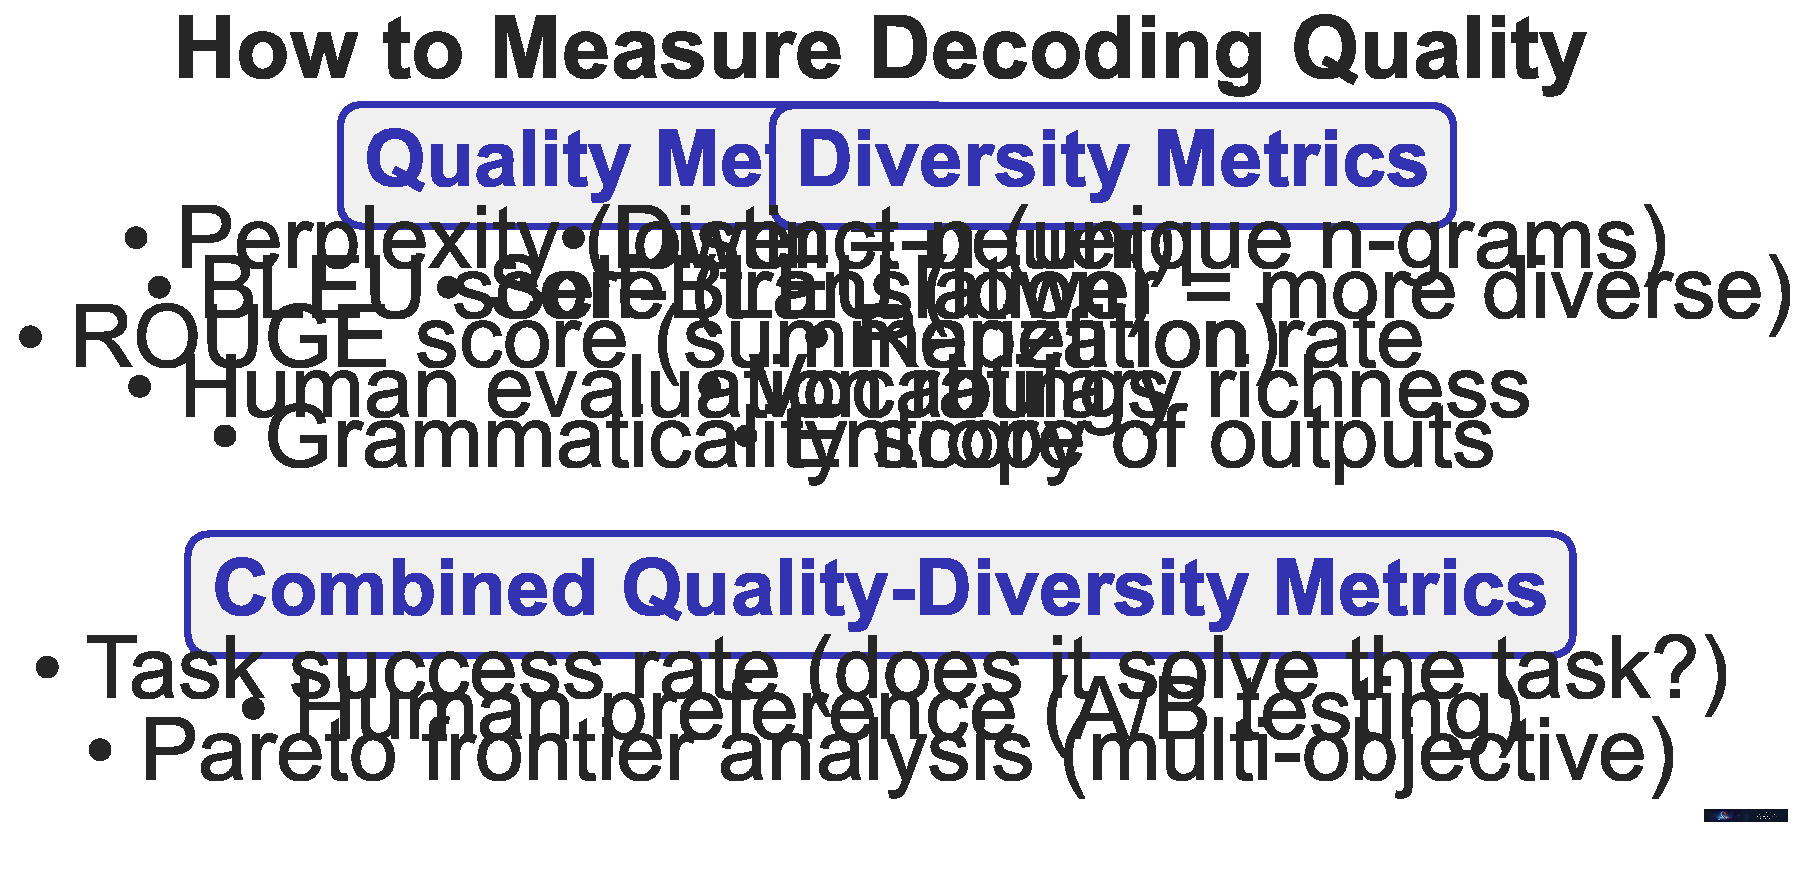
\includegraphics[width=0.65\textwidth]{../figures/quality_metrics_bsc.pdf}
\end{center}
\bottomnote{Need both quality AND diversity metrics}
\end{frame}

% === A11-A14: CONTRASTIVE & DEGENERATION ===

\begin{frame}[t]{A11: Degeneration Problem (Formal)}
\small
\textbf{Definition}: Unnatural repetitions in generated text

\vspace{2mm}
\textbf{Why It Happens}:

\begin{enumerate}
\item Model trained on natural text (low repetition)
\item Generation maximizes $P(y_t | y_{<t})$
\item Recent context influences $P$
\item Feedback loop: high prob → context → same high prob
\end{enumerate}

\vspace{2mm}
\colorbox{mlred!20}{\parbox{0.90\textwidth}{
\textbf{Quantifying}:

Greedy repetition: 15-30\%

Human text: 2-5\%

Gap = degeneration
}}

\vspace{2mm}
\textbf{Examples}: ``\textit{I think that I think that I think...}''

\bottomnote{Maximizing probability $\neq$ natural text}
\end{frame}

\begin{frame}[t]{A12: Contrastive Search Objective}
\small
\textbf{Scoring Function}:

$$\text{score}(w_t) = (1 - \alpha) \times P(w_t | y_{<t}) - \alpha \times \max_{w_i \in y_{<t}} \text{sim}(w_t, w_i)$$

where $\alpha \in [0, 1]$ controls tradeoff

\vspace{2mm}
\textbf{Similarity}: Cosine similarity using token embeddings

$$\text{sim}(w_i, w_j) = \frac{h_i \cdot h_j}{||h_i|| \cdot ||h_j||}$$

\vspace{2mm}
\textbf{Algorithm}:

\begin{enumerate}
\item Get top-k by probability
\item Compute similarity to all $y_{<t}$
\item Apply penalty: score = prob - $\alpha \times$ max\_sim
\item Select highest score
\end{enumerate}

\bottomnote{Explicit penalty for copying context}
\end{frame}

\begin{frame}[t]{A13: Contrastive Parameters}
\small
\begin{columns}[T]
\column{0.49\textwidth}
\textbf{Alpha} ($\alpha$):

$\alpha = 0$: Pure greedy

$\alpha = 0.6$: Balanced (default)

$\alpha = 1.0$: Max diversity

\vspace{2mm}
\textbf{Typical Settings}:

Short ($<$100): $\alpha = 0.4-0.5$

Medium ($<$500): $\alpha = 0.5-0.6$

Long (500+): $\alpha = 0.6-0.7$

\column{0.49\textwidth}
\textbf{Top-k} (candidates):

$k = 4$: Fast, focused

$k = 6$: Balanced (default)

$k = 10$: Diverse

\vspace{2mm}
\colorbox{mlred!20}{\parbox{0.85\textwidth}{
\textbf{Cost}: $O(k \times T^2)$

12× slower than greedy

Only for quality-critical
}}

\end{columns}
\bottomnote{Hugging Face default: $\alpha$=0.6, k=4}
\end{frame}

\begin{frame}[t]{A14: Degeneration Analysis (2024-2025)}
\small
\textbf{Research Findings}:

\begin{itemize}
\item Greedy: 18-25\% repetition (GPT-2), 12-18\% (GPT-3)
\item Nucleus: 8-12\% (still above human 3-5\%)
\item Contrastive: 4-7\% (closest to human)
\end{itemize}

\vspace{2mm}
\textbf{Why Probability Fails}:

Training: Next token prediction

Generation: Global coherence

Mismatch: Local optimum $\neq$ global quality

\vspace{2mm}
\colorbox{mllavender4}{\parbox{0.90\textwidth}{
\textbf{Solutions Hierarchy}:

1. Temp/Top-k/Nucleus: Reduce greedy determinism

2. Contrastive: Explicit penalty

3. RLHF/DPO: Align with humans (Week 10)
}}

\bottomnote{Contrastive addresses fundamental limitation}
\end{frame}

% === A15-A19: ADVANCED TOPICS ===

\begin{frame}[t]{A15: Hybrid Methods}
\small
\textbf{Combining Strategies}:

\vspace{2mm}
\textbf{Nucleus + Temperature}:

$$p_i(T) = \softmax(z / T), \text{ then } V_p \gets \text{nucleus}(p_i)$$

Used by GPT-3, ChatGPT

\vspace{2mm}
\textbf{Beam + Sampling}:

Beam search + stochastic selection

\vspace{2mm}
\textbf{Contrastive + Nucleus}:

Best of both worlds

\bottomnote{Hybrid methods leverage complementary strengths}
\end{frame}

\begin{frame}[t]{A16: Constrained Decoding (2025)}
\small
\textbf{Goal}: Force tokens/patterns

\vspace{2mm}
\textbf{Lexically Constrained}:

Must include keywords

Beam variant tracks satisfaction

\vspace{2mm}
\textbf{Format Constraints}:

JSON output, code syntax

\vspace{2mm}
\textbf{Use Cases}:

Structured extraction, controllable summarization, code generation

\bottomnote{Constrained decoding enables controllable generation}
\end{frame}

\begin{frame}[t]{A17: Computational Complexity}
\small
\begin{center}
\begin{tabular}{lccc}
\toprule
\textbf{Method} & \textbf{Time/token} & \textbf{Total} & \textbf{Speed} \\
\midrule
Greedy & $O(V)$ & $O(VT)$ & 1.0× \\
Temperature & $O(V)$ & $O(VT)$ & 1.1× \\
Top-k & $O(V)$ & $O(VT)$ & 1.2× \\
Nucleus & $O(V \log V)$ & $O(V \log V \cdot T)$ & 1.3× \\
Beam (k=5) & $O(kV)$ & $O(kVT)$ & 4.5× \\
Contrastive & $O(kT)$ & $O(kT^2)$ & 12× \\
\bottomrule
\end{tabular}
\end{center}

\vspace{2mm}
\colorbox{mllavender4}{\parbox{0.85\textwidth}{
\textbf{Practical} (1000 tokens):

Greedy: 2.5s | Nucleus: 3.2s | Beam: 11s | Contrastive: 30s
}}

\bottomnote{Computational cost matters for production}
\end{frame}

\begin{frame}[t]{A18: Production Settings (2024-2025)}
\vspace{-0.3cm}
\begin{center}
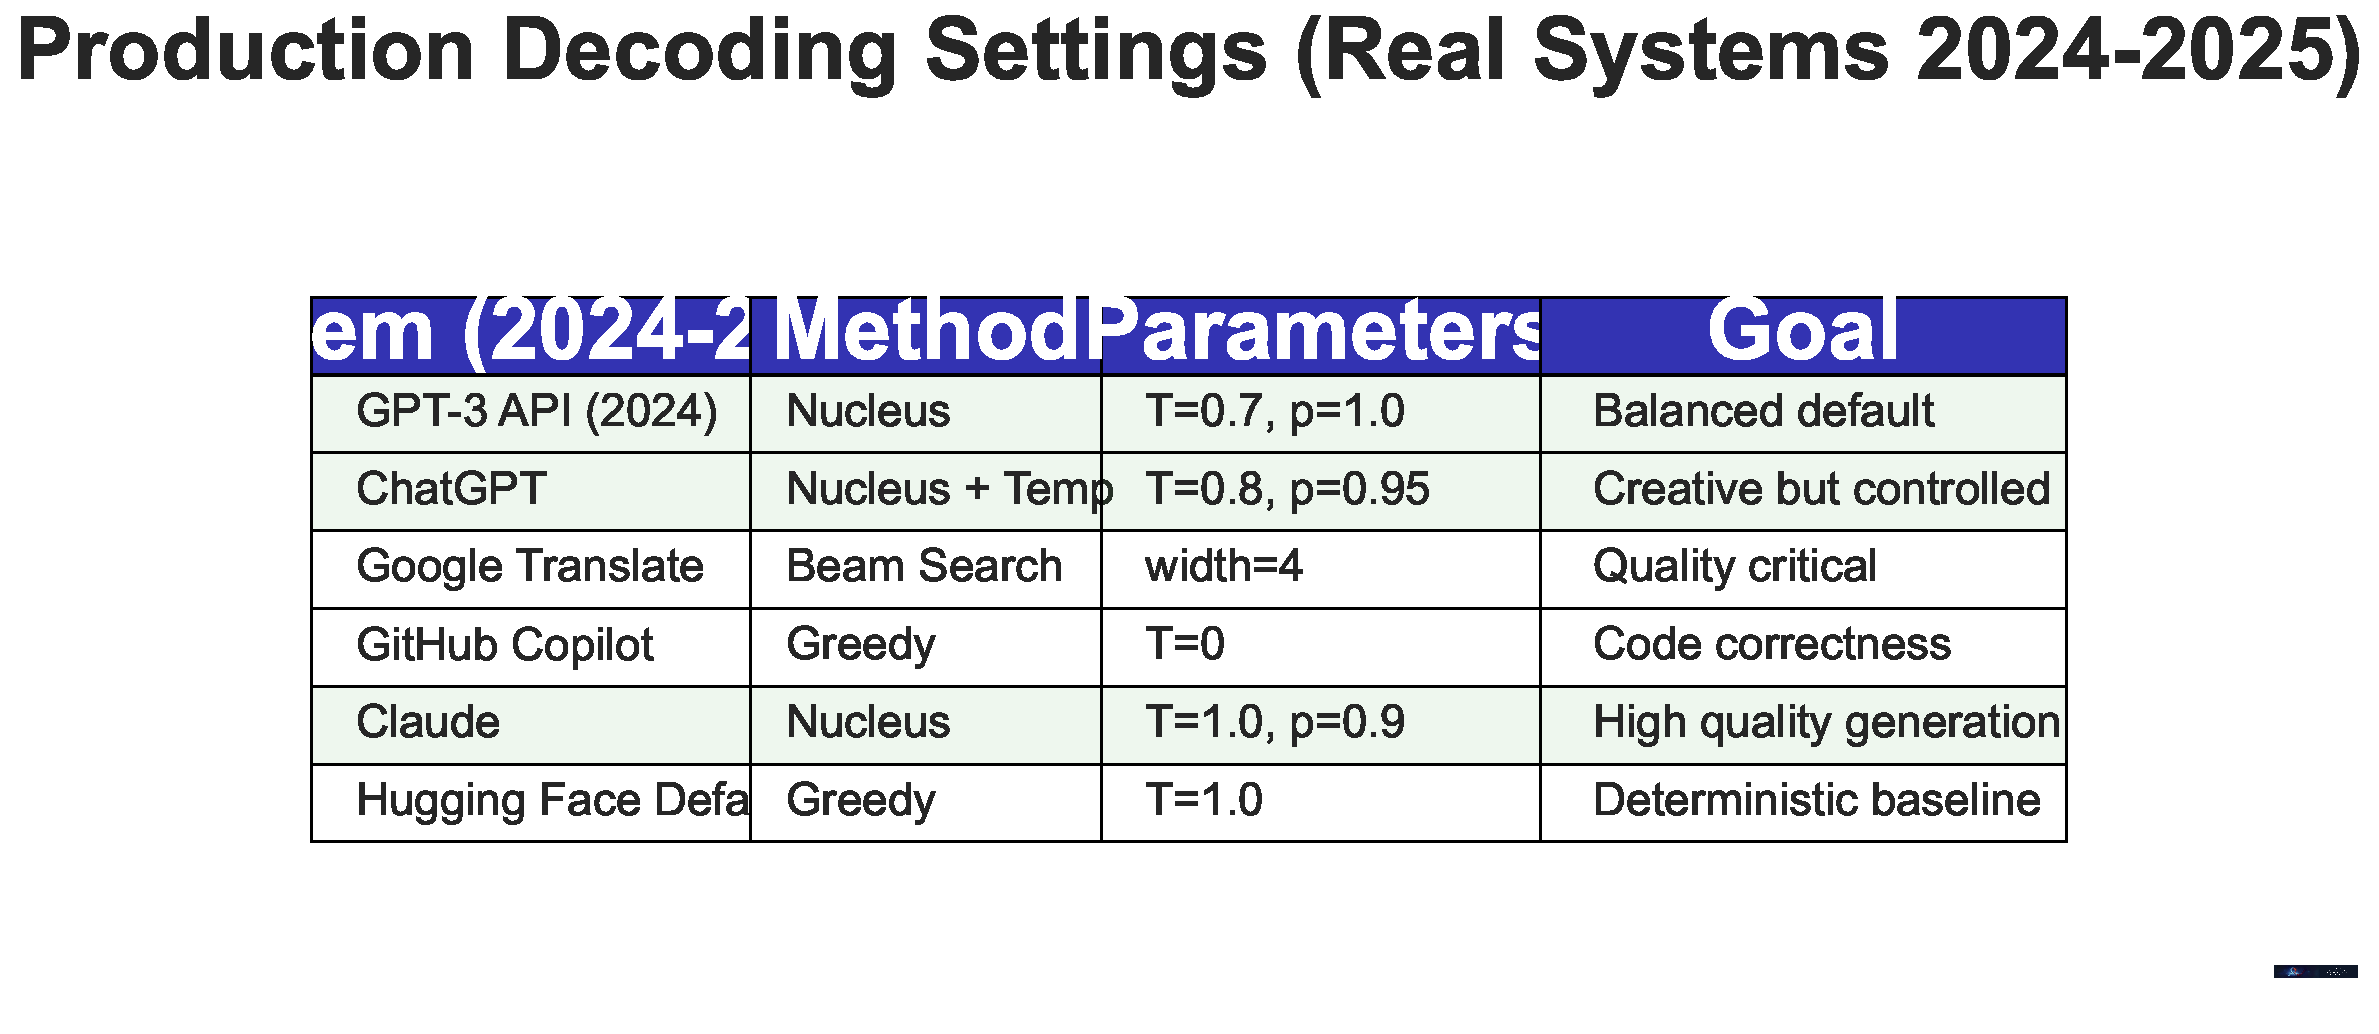
\includegraphics[width=0.75\textwidth]{../figures/production_settings_bsc.pdf}
\end{center}
\bottomnote{Real settings from major production systems}
\end{frame}

\begin{frame}[t]{A19: Future Directions (2025)}
\small
\textbf{Active Research}:

\begin{enumerate}
\item Quality-diversity optimization
\item Learned decoding (RLHF, DPO)
\item Speculative decoding (4-8× faster)
\item Adaptive methods
\item Energy-based decoding
\end{enumerate}

\vspace{2mm}
\colorbox{mllavender4}{\parbox{0.90\textwidth}{
\textbf{Open Problems}:

• Auto-select best parameters for new task?

• Balance fluency + factuality + creativity?

• Efficient 100K+ token decoding?
}}

\vspace{2mm}
\textbf{Trend}: Hand-tuned → learned decoding strategies

\bottomnote{Active research area with many open questions}
\end{frame}

\end{document}
